\documentclass[twoside]{book}

% Packages required by doxygen
\usepackage{fixltx2e}
\usepackage{calc}
\usepackage{doxygen}
\usepackage{graphicx}
\usepackage[utf8]{inputenc}
\usepackage{makeidx}
\usepackage{multicol}
\usepackage{multirow}
\PassOptionsToPackage{warn}{textcomp}
\usepackage{textcomp}
\usepackage[nointegrals]{wasysym}
\usepackage[table]{xcolor}

% Font selection
\usepackage[T1]{fontenc}
\usepackage{mathptmx}
\usepackage[scaled=.90]{helvet}
\usepackage{courier}
\usepackage{amssymb}
\usepackage{sectsty}
\renewcommand{\familydefault}{\sfdefault}
\allsectionsfont{%
  \fontseries{bc}\selectfont%
  \color{darkgray}%
}
\renewcommand{\DoxyLabelFont}{%
  \fontseries{bc}\selectfont%
  \color{darkgray}%
}
\newcommand{\+}{\discretionary{\mbox{\scriptsize$\hookleftarrow$}}{}{}}

% Page & text layout
\usepackage{geometry}
\geometry{%
  a4paper,%
  top=2.5cm,%
  bottom=2.5cm,%
  left=2.5cm,%
  right=2.5cm%
}
\tolerance=750
\hfuzz=15pt
\hbadness=750
\setlength{\emergencystretch}{15pt}
\setlength{\parindent}{0cm}
\setlength{\parskip}{0.2cm}
\makeatletter
\renewcommand{\paragraph}{%
  \@startsection{paragraph}{4}{0ex}{-1.0ex}{1.0ex}{%
    \normalfont\normalsize\bfseries\SS@parafont%
  }%
}
\renewcommand{\subparagraph}{%
  \@startsection{subparagraph}{5}{0ex}{-1.0ex}{1.0ex}{%
    \normalfont\normalsize\bfseries\SS@subparafont%
  }%
}
\makeatother

% Headers & footers
\usepackage{fancyhdr}
\pagestyle{fancyplain}
\fancyhead[LE]{\fancyplain{}{\bfseries\thepage}}
\fancyhead[CE]{\fancyplain{}{}}
\fancyhead[RE]{\fancyplain{}{\bfseries\leftmark}}
\fancyhead[LO]{\fancyplain{}{\bfseries\rightmark}}
\fancyhead[CO]{\fancyplain{}{}}
\fancyhead[RO]{\fancyplain{}{\bfseries\thepage}}
\fancyfoot[LE]{\fancyplain{}{}}
\fancyfoot[CE]{\fancyplain{}{}}
\fancyfoot[RE]{\fancyplain{}{\bfseries\scriptsize Generated on Tue Feb 21 2017 21\+:43\+:32 for My Project by Doxygen }}
\fancyfoot[LO]{\fancyplain{}{\bfseries\scriptsize Generated on Tue Feb 21 2017 21\+:43\+:32 for My Project by Doxygen }}
\fancyfoot[CO]{\fancyplain{}{}}
\fancyfoot[RO]{\fancyplain{}{}}
\renewcommand{\footrulewidth}{0.4pt}
\renewcommand{\chaptermark}[1]{%
  \markboth{#1}{}%
}
\renewcommand{\sectionmark}[1]{%
  \markright{\thesection\ #1}%
}

% Indices & bibliography
\usepackage{natbib}
\usepackage[titles]{tocloft}
\setcounter{tocdepth}{3}
\setcounter{secnumdepth}{5}
\makeindex

% Hyperlinks (required, but should be loaded last)
\usepackage{ifpdf}
\ifpdf
  \usepackage[pdftex,pagebackref=true]{hyperref}
\else
  \usepackage[ps2pdf,pagebackref=true]{hyperref}
\fi
\hypersetup{%
  colorlinks=true,%
  linkcolor=blue,%
  citecolor=blue,%
  unicode%
}

% Custom commands
\newcommand{\clearemptydoublepage}{%
  \newpage{\pagestyle{empty}\cleardoublepage}%
}


%===== C O N T E N T S =====

\begin{document}

% Titlepage & ToC
\hypersetup{pageanchor=false,
             bookmarks=true,
             bookmarksnumbered=true,
             pdfencoding=unicode
            }
\pagenumbering{roman}
\begin{titlepage}
\vspace*{7cm}
\begin{center}%
{\Large My Project }\\
\vspace*{1cm}
{\large Generated by Doxygen 1.8.8}\\
\vspace*{0.5cm}
{\small Tue Feb 21 2017 21:43:32}\\
\end{center}
\end{titlepage}
\clearemptydoublepage
\tableofcontents
\clearemptydoublepage
\pagenumbering{arabic}
\hypersetup{pageanchor=true}

%--- Begin generated contents ---
\chapter{Hierarchical Index}
\section{Class Hierarchy}
This inheritance list is sorted roughly, but not completely, alphabetically\+:\begin{DoxyCompactList}
\item \contentsline{section}{Client}{\pageref{classClient}}{}
\item J\+Frame\begin{DoxyCompactList}
\item \contentsline{section}{Myframe}{\pageref{classMyframe}}{}
\end{DoxyCompactList}
\end{DoxyCompactList}

\chapter{Class Index}
\section{Class List}
Here are the classes, structs, unions and interfaces with brief descriptions\+:\begin{DoxyCompactList}
\item\contentsline{section}{\hyperlink{structcppu_1_1TCPServer_1_1Callback}{cppu\+::\+T\+C\+P\+Server\+::\+Callback} \\*\hyperlink{structcppu_1_1TCPServer_1_1Callback}{Callback} interface }{\pageref{structcppu_1_1TCPServer_1_1Callback}}{}
\item\contentsline{section}{\hyperlink{structcppu_1_1TCPServer_1_1CallbackMethod}{cppu\+::\+T\+C\+P\+Server\+::\+Callback\+Method$<$ T $>$} }{\pageref{structcppu_1_1TCPServer_1_1CallbackMethod}}{}
\item\contentsline{section}{\hyperlink{classFactory}{Factory} }{\pageref{classFactory}}{}
\item\contentsline{section}{\hyperlink{classFilm}{Film} }{\pageref{classFilm}}{}
\item\contentsline{section}{\hyperlink{structcppu_1_1InputBuffer}{cppu\+::\+Input\+Buffer} }{\pageref{structcppu_1_1InputBuffer}}{}
\item\contentsline{section}{\hyperlink{classListMedia}{List\+Media$<$ T $>$} }{\pageref{classListMedia}}{}
\item\contentsline{section}{\hyperlink{classMultimedia}{Multimedia} }{\pageref{classMultimedia}}{}
\item\contentsline{section}{\hyperlink{classMyBase}{My\+Base} }{\pageref{classMyBase}}{}
\item\contentsline{section}{\hyperlink{classPhoto}{Photo} }{\pageref{classPhoto}}{}
\item\contentsline{section}{\hyperlink{classcppu_1_1ServerSocket}{cppu\+::\+Server\+Socket} \\*T\+C\+P/\+I\+P server socket. This class implements a T\+C\+P/\+I\+P socket that waits for requests to come in over the network. A\+F\+\_\+\+I\+N\+E\+T connections following the I\+Pv4 Internet protocol are supported }{\pageref{classcppu_1_1ServerSocket}}{}
\item\contentsline{section}{\hyperlink{classcppu_1_1Socket}{cppu\+::\+Socket} \\*T\+C\+P/\+I\+P or U\+D\+P/\+Datagram socket. This class encapsulates a T\+C\+P/\+I\+P or U\+D\+P/\+Datagram socket. A\+F\+\_\+\+I\+N\+E\+T connections following the I\+Pv4 Internet protocol are supported }{\pageref{classcppu_1_1Socket}}{}
\item\contentsline{section}{\hyperlink{classcppu_1_1SocketBuffer}{cppu\+::\+Socket\+Buffer} \\*Preserves record boundaries when exchanging data between connected T\+C\+P/\+I\+P sockets. This class ensures that one call to \hyperlink{classcppu_1_1SocketBuffer_a92ae0351aaee8719d34e8c4618495d59}{write\+Line()} corresponds to one and exactly one call to \hyperlink{classcppu_1_1SocketBuffer_a222769d3776b9cbd3a727ee1f0e60358}{read\+Line()} on the other side. This differs from the behavior of \hyperlink{classcppu_1_1Socket_aeac77f859159715e2d63a5a0dc118788}{Socket\+::send()} and \hyperlink{classcppu_1_1Socket_a37c382af52cc02f92c0e19a0c6e0e04f}{Socket\+::receive()} because T\+C\+P/\+I\+P connected sockets do not preserve record boundaries. \hyperlink{classcppu_1_1SocketBuffer_a92ae0351aaee8719d34e8c4618495d59}{write\+Line()} and \hyperlink{classcppu_1_1SocketBuffer_a222769d3776b9cbd3a727ee1f0e60358}{read\+Line()} solve this problem by automatically adding and searching for a separator between successive lines }{\pageref{classcppu_1_1SocketBuffer}}{}
\item\contentsline{section}{\hyperlink{classcppu_1_1TCPConnection}{cppu\+::\+T\+C\+P\+Connection} \\*Connection with a given client. Each \hyperlink{classcppu_1_1TCPConnection}{T\+C\+P\+Connection} uses a different thread }{\pageref{classcppu_1_1TCPConnection}}{}
\item\contentsline{section}{\hyperlink{classcppu_1_1TCPLock}{cppu\+::\+T\+C\+P\+Lock} \\*Locks the server in read mode or in write mode. Must be created {\itshape in the stack} by the callback method }{\pageref{classcppu_1_1TCPLock}}{}
\item\contentsline{section}{\hyperlink{classcppu_1_1TCPServer}{cppu\+::\+T\+C\+P\+Server} \\*T\+C\+P/\+I\+P I\+Pv4 server. The server supports T\+C\+P/\+I\+P A\+F\+\_\+\+I\+N\+E\+T connections (following the I\+Pv4 Internet protocol) with multiple clients. One thread is used per client }{\pageref{classcppu_1_1TCPServer}}{}
\item\contentsline{section}{\hyperlink{classVideo}{Video} }{\pageref{classVideo}}{}
\end{DoxyCompactList}

\chapter{Class Documentation}
\hypertarget{structcppu_1_1TCPServer_1_1Callback}{\section{cppu\+:\+:T\+C\+P\+Server\+:\+:Callback Struct Reference}
\label{structcppu_1_1TCPServer_1_1Callback}\index{cppu\+::\+T\+C\+P\+Server\+::\+Callback@{cppu\+::\+T\+C\+P\+Server\+::\+Callback}}
}


\hyperlink{structcppu_1_1TCPServer_1_1Callback}{Callback} interface.  




{\ttfamily \#include $<$tcpserver.\+h$>$}



Inheritance diagram for cppu\+:\+:T\+C\+P\+Server\+:\+:Callback\+:
\nopagebreak
\begin{figure}[H]
\begin{center}
\leavevmode
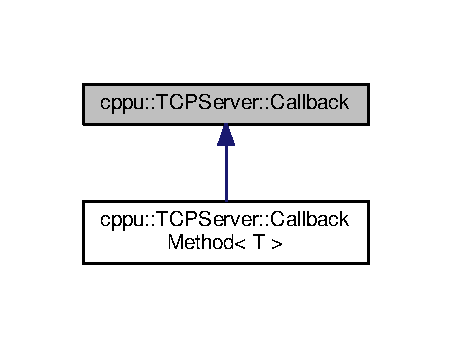
\includegraphics[width=217pt]{structcppu_1_1TCPServer_1_1Callback__inherit__graph}
\end{center}
\end{figure}
\subsection*{Public Member Functions}
\begin{DoxyCompactItemize}
\item 
\hypertarget{structcppu_1_1TCPServer_1_1Callback_aabe4b0b30e14ddeb7c0c02aa3a335eba}{virtual bool {\bfseries call} (\hyperlink{classcppu_1_1TCPConnection}{T\+C\+P\+Connection} \&cnx, const std\+::string \&request, std\+::string \&response)=0}\label{structcppu_1_1TCPServer_1_1Callback_aabe4b0b30e14ddeb7c0c02aa3a335eba}

\end{DoxyCompactItemize}


\subsection{Detailed Description}
\hyperlink{structcppu_1_1TCPServer_1_1Callback}{Callback} interface. 

The documentation for this struct was generated from the following file\+:\begin{DoxyCompactItemize}
\item 
tcpserver.\+h\end{DoxyCompactItemize}

\hypertarget{structcppu_1_1TCPServer_1_1CallbackMethod}{\section{cppu\+:\+:T\+C\+P\+Server\+:\+:Callback\+Method$<$ T $>$ Struct Template Reference}
\label{structcppu_1_1TCPServer_1_1CallbackMethod}\index{cppu\+::\+T\+C\+P\+Server\+::\+Callback\+Method$<$ T $>$@{cppu\+::\+T\+C\+P\+Server\+::\+Callback\+Method$<$ T $>$}}
}


Inheritance diagram for cppu\+:\+:T\+C\+P\+Server\+:\+:Callback\+Method$<$ T $>$\+:
\nopagebreak
\begin{figure}[H]
\begin{center}
\leavevmode
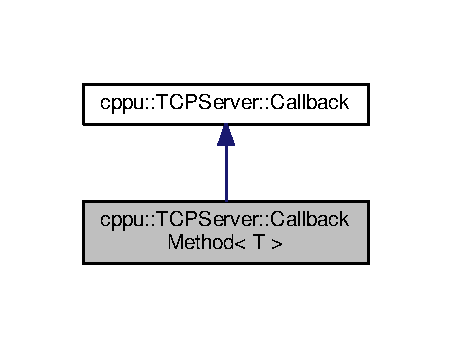
\includegraphics[width=217pt]{structcppu_1_1TCPServer_1_1CallbackMethod__inherit__graph}
\end{center}
\end{figure}


Collaboration diagram for cppu\+:\+:T\+C\+P\+Server\+:\+:Callback\+Method$<$ T $>$\+:
\nopagebreak
\begin{figure}[H]
\begin{center}
\leavevmode
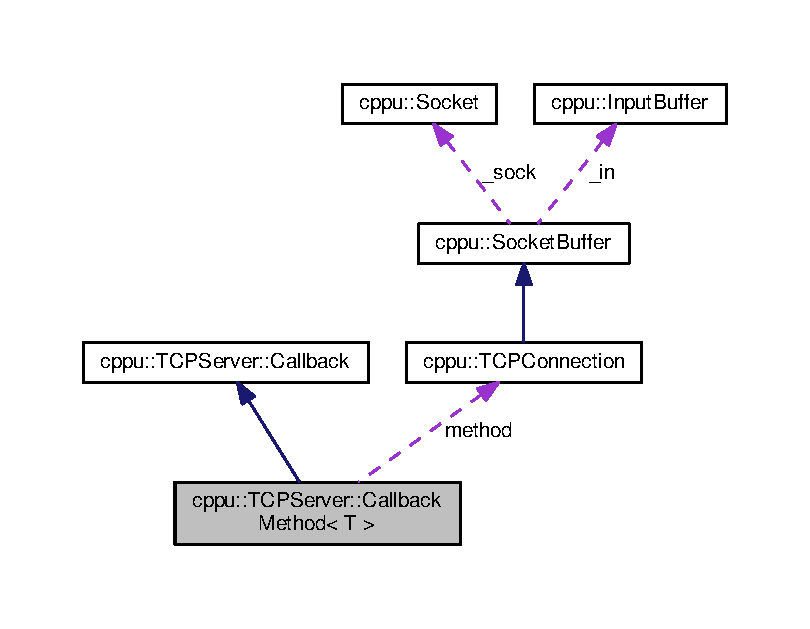
\includegraphics[width=350pt]{structcppu_1_1TCPServer_1_1CallbackMethod__coll__graph}
\end{center}
\end{figure}
\subsection*{Public Types}
\begin{DoxyCompactItemize}
\item 
\hypertarget{structcppu_1_1TCPServer_1_1CallbackMethod_a2911cc72786a989aa57c660248ffb44c}{typedef bool(T\+::$\ast$ {\bfseries Fun} )(\hyperlink{classcppu_1_1TCPConnection}{T\+C\+P\+Connection} \&, const std\+::string \&, std\+::string \&)}\label{structcppu_1_1TCPServer_1_1CallbackMethod_a2911cc72786a989aa57c660248ffb44c}

\end{DoxyCompactItemize}
\subsection*{Public Member Functions}
\begin{DoxyCompactItemize}
\item 
\hypertarget{structcppu_1_1TCPServer_1_1CallbackMethod_a0c6ceee6db8c67ef56fb26d1df52140f}{{\bfseries Callback\+Method} (T \&obj, Fun method)}\label{structcppu_1_1TCPServer_1_1CallbackMethod_a0c6ceee6db8c67ef56fb26d1df52140f}

\item 
\hypertarget{structcppu_1_1TCPServer_1_1CallbackMethod_a0c11039d0ed983c03a614d0764df3793}{virtual bool {\bfseries call} (\hyperlink{classcppu_1_1TCPConnection}{T\+C\+P\+Connection} \&cnx, const std\+::string \&req, std\+::string \&resp)}\label{structcppu_1_1TCPServer_1_1CallbackMethod_a0c11039d0ed983c03a614d0764df3793}

\end{DoxyCompactItemize}
\subsection*{Public Attributes}
\begin{DoxyCompactItemize}
\item 
\hypertarget{structcppu_1_1TCPServer_1_1CallbackMethod_ae480535d346efc119fb5c43880f349c8}{T \& {\bfseries obj}}\label{structcppu_1_1TCPServer_1_1CallbackMethod_ae480535d346efc119fb5c43880f349c8}

\item 
\hypertarget{structcppu_1_1TCPServer_1_1CallbackMethod_aab858a039ddee71fb65a0e35c173f067}{Fun {\bfseries method}}\label{structcppu_1_1TCPServer_1_1CallbackMethod_aab858a039ddee71fb65a0e35c173f067}

\end{DoxyCompactItemize}


The documentation for this struct was generated from the following file\+:\begin{DoxyCompactItemize}
\item 
tcpserver.\+h\end{DoxyCompactItemize}

\hypertarget{classFactory}{\section{Factory Class Reference}
\label{classFactory}\index{Factory@{Factory}}
}
\subsection*{Public Member Functions}
\begin{DoxyCompactItemize}
\item 
\hyperlink{classFactory_ac792bf88cfb7b6804b479529da5308cc}{Factory} ()
\begin{DoxyCompactList}\small\item\em \hyperlink{classFactory}{Factory}. \end{DoxyCompactList}\item 
virtual Photo\+Ptr \hyperlink{classFactory_adceba4e3ec5f562f8c763df4a4867e5c}{create\+Photo} (string \+\_\+nom\+F=\char`\"{}\char`\"{}, string \+\_\+nom\+M=\char`\"{}\char`\"{}, double \+\_\+latitude=0, double \+\_\+longitude=0)
\begin{DoxyCompactList}\small\item\em create\+Photo \end{DoxyCompactList}\item 
virtual Video\+Ptr \hyperlink{classFactory_af9d206c8e60d86c56b00d16edcc5bf4d}{create\+Video} (string \+\_\+nom\+F=\char`\"{}\char`\"{}, string \+\_\+nom\+M=\char`\"{}\char`\"{}, int \+\_\+duree=0)
\begin{DoxyCompactList}\small\item\em create\+Video \end{DoxyCompactList}\item 
virtual Film\+Ptr \hyperlink{classFactory_aa123d5c1891fe01e10b529e6569fa867}{create\+Film} (string \+\_\+nom\+F=\char`\"{}\char`\"{}, string \+\_\+nom\+M=\char`\"{}\char`\"{}, int \+\_\+duree=0, int $\ast$\+\_\+chap=0, int \+\_\+num\+\_\+chap=0)
\begin{DoxyCompactList}\small\item\em create\+Film \end{DoxyCompactList}\item 
virtual List\+Media\+Ptr$<$ Media\+Ptr $>$ \hyperlink{classFactory_a76454621c8e60b827df3b2ef12160a19}{create\+List} (string \+\_\+name=\char`\"{}\char`\"{})
\begin{DoxyCompactList}\small\item\em create\+List \end{DoxyCompactList}\item 
virtual Media\+Ptr \hyperlink{classFactory_aee81375a6edf8dc3ed02f00ff62c03d1}{display\+Media\+By\+Name} (string \+\_\+nom, ostream \&out) const 
\begin{DoxyCompactList}\small\item\em display\+Media\+By\+Name \end{DoxyCompactList}\item 
virtual List\+Media\+Ptr$<$ Media\+Ptr $>$ \hyperlink{classFactory_a7c2411c0b661abf2f3723d926ad49079}{display\+Group\+By\+Name} (string \+\_\+nom, ostream \&out) const 
\begin{DoxyCompactList}\small\item\em display\+Group\+By\+Name \end{DoxyCompactList}\item 
virtual void \hyperlink{classFactory_a53452fb77521c5194c4820953475d9d9}{play\+By\+Name} (string \+\_\+nom) const 
\begin{DoxyCompactList}\small\item\em play\+By\+Name \end{DoxyCompactList}\item 
virtual void \hyperlink{classFactory_a3ec2b831092fb60da2fb0b713923d5f1}{read\+File} (ifstream \&fs)
\begin{DoxyCompactList}\small\item\em read\+File \end{DoxyCompactList}\item 
virtual void \hyperlink{classFactory_a4e8a61786c5fac01938808801cb30ff9}{save\+File} (ofstream \&fs)
\begin{DoxyCompactList}\small\item\em save\+File \end{DoxyCompactList}\item 
virtual void \hyperlink{classFactory_ac806b24675e7d9c1f2f021cb346c65ea}{display\+All\+Media} (ostream \&out)
\begin{DoxyCompactList}\small\item\em display\+All\+Media \end{DoxyCompactList}\end{DoxyCompactItemize}


\subsection{Constructor \& Destructor Documentation}
\hypertarget{classFactory_ac792bf88cfb7b6804b479529da5308cc}{\index{Factory@{Factory}!Factory@{Factory}}
\index{Factory@{Factory}!Factory@{Factory}}
\subsubsection[{Factory}]{\setlength{\rightskip}{0pt plus 5cm}Factory\+::\+Factory (
\begin{DoxyParamCaption}
{}
\end{DoxyParamCaption}
)}}\label{classFactory_ac792bf88cfb7b6804b479529da5308cc}


\hyperlink{classFactory}{Factory}. 


\begin{DoxyParams}{Parameters}
{\em } & return  Create a ifstream and read the media in the \char`\"{}dict\+\_\+m.\+txt\char`\"{} \\
\hline
\end{DoxyParams}


\subsection{Member Function Documentation}
\hypertarget{classFactory_aa123d5c1891fe01e10b529e6569fa867}{\index{Factory@{Factory}!create\+Film@{create\+Film}}
\index{create\+Film@{create\+Film}!Factory@{Factory}}
\subsubsection[{create\+Film}]{\setlength{\rightskip}{0pt plus 5cm}Film\+Ptr Factory\+::create\+Film (
\begin{DoxyParamCaption}
\item[{string}]{\+\_\+nom\+F = {\ttfamily \char`\"{}\char`\"{}}, }
\item[{string}]{\+\_\+nom\+M = {\ttfamily \char`\"{}\char`\"{}}, }
\item[{int}]{\+\_\+duree = {\ttfamily 0}, }
\item[{int $\ast$}]{\+\_\+chap = {\ttfamily 0}, }
\item[{int}]{\+\_\+num\+\_\+chap = {\ttfamily 0}}
\end{DoxyParamCaption}
)\hspace{0.3cm}{\ttfamily [virtual]}}}\label{classFactory_aa123d5c1891fe01e10b529e6569fa867}


create\+Film 


\begin{DoxyParams}{Parameters}
{\em \+\_\+nom\+F,\+\_\+nom\+M,\+\_\+duree,$\ast$\+\_\+chap,\+\_\+num\+\_\+chap} & \\
\hline
\end{DoxyParams}
\begin{DoxyReturn}{Returns}
film  Create a film with the parameters, return a smart pointer of film 
\end{DoxyReturn}
\hypertarget{classFactory_a76454621c8e60b827df3b2ef12160a19}{\index{Factory@{Factory}!create\+List@{create\+List}}
\index{create\+List@{create\+List}!Factory@{Factory}}
\subsubsection[{create\+List}]{\setlength{\rightskip}{0pt plus 5cm}List\+Media\+Ptr$<$ Media\+Ptr $>$ Factory\+::create\+List (
\begin{DoxyParamCaption}
\item[{string}]{\+\_\+name = {\ttfamily \char`\"{}\char`\"{}}}
\end{DoxyParamCaption}
)\hspace{0.3cm}{\ttfamily [virtual]}}}\label{classFactory_a76454621c8e60b827df3b2ef12160a19}


create\+List 


\begin{DoxyParams}{Parameters}
{\em \+\_\+name} & \\
\hline
\end{DoxyParams}
\begin{DoxyReturn}{Returns}
listmedia  Create a listmedia with the parameters, return a smart pointer of listmedia 
\end{DoxyReturn}
\hypertarget{classFactory_adceba4e3ec5f562f8c763df4a4867e5c}{\index{Factory@{Factory}!create\+Photo@{create\+Photo}}
\index{create\+Photo@{create\+Photo}!Factory@{Factory}}
\subsubsection[{create\+Photo}]{\setlength{\rightskip}{0pt plus 5cm}Photo\+Ptr Factory\+::create\+Photo (
\begin{DoxyParamCaption}
\item[{string}]{\+\_\+nom\+F = {\ttfamily \char`\"{}\char`\"{}}, }
\item[{string}]{\+\_\+nom\+M = {\ttfamily \char`\"{}\char`\"{}}, }
\item[{double}]{\+\_\+latitude = {\ttfamily 0}, }
\item[{double}]{\+\_\+longitude = {\ttfamily 0}}
\end{DoxyParamCaption}
)\hspace{0.3cm}{\ttfamily [virtual]}}}\label{classFactory_adceba4e3ec5f562f8c763df4a4867e5c}


create\+Photo 


\begin{DoxyParams}{Parameters}
{\em \+\_\+nom\+F,\+\_\+nom\+M,\+\_\+latitude,\+\_\+longitude} & \\
\hline
\end{DoxyParams}
\begin{DoxyReturn}{Returns}
photo  Create a photo with the parameters, return a smart pointer of photo 
\end{DoxyReturn}
\hypertarget{classFactory_af9d206c8e60d86c56b00d16edcc5bf4d}{\index{Factory@{Factory}!create\+Video@{create\+Video}}
\index{create\+Video@{create\+Video}!Factory@{Factory}}
\subsubsection[{create\+Video}]{\setlength{\rightskip}{0pt plus 5cm}Video\+Ptr Factory\+::create\+Video (
\begin{DoxyParamCaption}
\item[{string}]{\+\_\+nom\+F = {\ttfamily \char`\"{}\char`\"{}}, }
\item[{string}]{\+\_\+nom\+M = {\ttfamily \char`\"{}\char`\"{}}, }
\item[{int}]{\+\_\+duree = {\ttfamily 0}}
\end{DoxyParamCaption}
)\hspace{0.3cm}{\ttfamily [virtual]}}}\label{classFactory_af9d206c8e60d86c56b00d16edcc5bf4d}


create\+Video 


\begin{DoxyParams}{Parameters}
{\em \+\_\+nom\+F,\+\_\+nom\+M,\+\_\+duree} & \\
\hline
\end{DoxyParams}
\begin{DoxyReturn}{Returns}
video  Create a video with the parameters, return a smart pointer of video 
\end{DoxyReturn}
\hypertarget{classFactory_ac806b24675e7d9c1f2f021cb346c65ea}{\index{Factory@{Factory}!display\+All\+Media@{display\+All\+Media}}
\index{display\+All\+Media@{display\+All\+Media}!Factory@{Factory}}
\subsubsection[{display\+All\+Media}]{\setlength{\rightskip}{0pt plus 5cm}void Factory\+::display\+All\+Media (
\begin{DoxyParamCaption}
\item[{ostream \&}]{out}
\end{DoxyParamCaption}
)\hspace{0.3cm}{\ttfamily [virtual]}}}\label{classFactory_ac806b24675e7d9c1f2f021cb346c65ea}


display\+All\+Media 


\begin{DoxyParams}{Parameters}
{\em out} & \\
\hline
\end{DoxyParams}
\begin{DoxyReturn}{Returns}
display all the media 
\end{DoxyReturn}
\hypertarget{classFactory_a7c2411c0b661abf2f3723d926ad49079}{\index{Factory@{Factory}!display\+Group\+By\+Name@{display\+Group\+By\+Name}}
\index{display\+Group\+By\+Name@{display\+Group\+By\+Name}!Factory@{Factory}}
\subsubsection[{display\+Group\+By\+Name}]{\setlength{\rightskip}{0pt plus 5cm}List\+Media\+Ptr$<$ Media\+Ptr $>$ Factory\+::display\+Group\+By\+Name (
\begin{DoxyParamCaption}
\item[{string}]{\+\_\+nom, }
\item[{ostream \&}]{out}
\end{DoxyParamCaption}
) const\hspace{0.3cm}{\ttfamily [virtual]}}}\label{classFactory_a7c2411c0b661abf2f3723d926ad49079}


display\+Group\+By\+Name 


\begin{DoxyParams}{Parameters}
{\em \+\_\+nom,out} & \\
\hline
\end{DoxyParams}
\begin{DoxyReturn}{Returns}
the smart pointer of found group  show the information of a group(given a name of group) 
\end{DoxyReturn}
\hypertarget{classFactory_aee81375a6edf8dc3ed02f00ff62c03d1}{\index{Factory@{Factory}!display\+Media\+By\+Name@{display\+Media\+By\+Name}}
\index{display\+Media\+By\+Name@{display\+Media\+By\+Name}!Factory@{Factory}}
\subsubsection[{display\+Media\+By\+Name}]{\setlength{\rightskip}{0pt plus 5cm}Media\+Ptr Factory\+::display\+Media\+By\+Name (
\begin{DoxyParamCaption}
\item[{string}]{\+\_\+nom, }
\item[{ostream \&}]{out}
\end{DoxyParamCaption}
) const\hspace{0.3cm}{\ttfamily [virtual]}}}\label{classFactory_aee81375a6edf8dc3ed02f00ff62c03d1}


display\+Media\+By\+Name 


\begin{DoxyParams}{Parameters}
{\em \+\_\+nom,out} & \\
\hline
\end{DoxyParams}
\begin{DoxyReturn}{Returns}
the smart pointer of found media  show the information of a media(given a name of media) 
\end{DoxyReturn}
\hypertarget{classFactory_a53452fb77521c5194c4820953475d9d9}{\index{Factory@{Factory}!play\+By\+Name@{play\+By\+Name}}
\index{play\+By\+Name@{play\+By\+Name}!Factory@{Factory}}
\subsubsection[{play\+By\+Name}]{\setlength{\rightskip}{0pt plus 5cm}void Factory\+::play\+By\+Name (
\begin{DoxyParamCaption}
\item[{string}]{\+\_\+nom}
\end{DoxyParamCaption}
) const\hspace{0.3cm}{\ttfamily [virtual]}}}\label{classFactory_a53452fb77521c5194c4820953475d9d9}


play\+By\+Name 


\begin{DoxyParams}{Parameters}
{\em \+\_\+nom} & \\
\hline
\end{DoxyParams}
\begin{DoxyReturn}{Returns}
show a media(given a name of group) 
\end{DoxyReturn}
\hypertarget{classFactory_a3ec2b831092fb60da2fb0b713923d5f1}{\index{Factory@{Factory}!read\+File@{read\+File}}
\index{read\+File@{read\+File}!Factory@{Factory}}
\subsubsection[{read\+File}]{\setlength{\rightskip}{0pt plus 5cm}void Factory\+::read\+File (
\begin{DoxyParamCaption}
\item[{ifstream \&}]{fs}
\end{DoxyParamCaption}
)\hspace{0.3cm}{\ttfamily [virtual]}}}\label{classFactory_a3ec2b831092fb60da2fb0b713923d5f1}


read\+File 


\begin{DoxyParams}{Parameters}
{\em fs} & \\
\hline
\end{DoxyParams}
\begin{DoxyReturn}{Returns}
read the media into the ofstream 
\end{DoxyReturn}
\hypertarget{classFactory_a4e8a61786c5fac01938808801cb30ff9}{\index{Factory@{Factory}!save\+File@{save\+File}}
\index{save\+File@{save\+File}!Factory@{Factory}}
\subsubsection[{save\+File}]{\setlength{\rightskip}{0pt plus 5cm}void Factory\+::save\+File (
\begin{DoxyParamCaption}
\item[{ofstream \&}]{fs}
\end{DoxyParamCaption}
)\hspace{0.3cm}{\ttfamily [virtual]}}}\label{classFactory_a4e8a61786c5fac01938808801cb30ff9}


save\+File 


\begin{DoxyParams}{Parameters}
{\em fs} & \\
\hline
\end{DoxyParams}
\begin{DoxyReturn}{Returns}
save the media into the ofstream 
\end{DoxyReturn}


The documentation for this class was generated from the following files\+:\begin{DoxyCompactItemize}
\item 
factory.\+h\item 
factory.\+cpp\end{DoxyCompactItemize}

\hypertarget{classFilm}{\section{Film Class Reference}
\label{classFilm}\index{Film@{Film}}
}


Inheritance diagram for Film\+:
\nopagebreak
\begin{figure}[H]
\begin{center}
\leavevmode
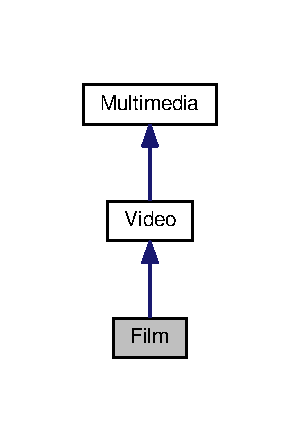
\includegraphics[width=144pt]{classFilm__inherit__graph}
\end{center}
\end{figure}


Collaboration diagram for Film\+:
\nopagebreak
\begin{figure}[H]
\begin{center}
\leavevmode
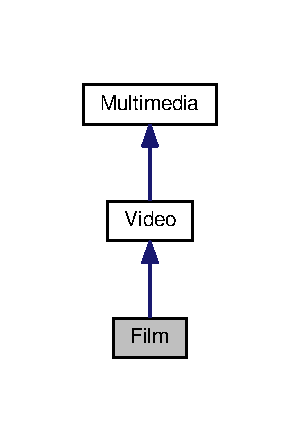
\includegraphics[width=144pt]{classFilm__coll__graph}
\end{center}
\end{figure}
\subsection*{Public Member Functions}
\begin{DoxyCompactItemize}
\item 
\hyperlink{classFilm_ac27cea51ddd9ba34caa4e3b7c57c1135}{Film} (string \+\_\+nom\+F=\char`\"{}\char`\"{}, string \+\_\+nom\+M=\char`\"{}\char`\"{}, int \+\_\+duree=0, int $\ast$\+\_\+chap=0, int \+\_\+num\+\_\+chap=0)
\begin{DoxyCompactList}\small\item\em \hyperlink{classFilm}{Film}. \end{DoxyCompactList}\item 
virtual \hyperlink{classFilm_a8dab653f8a6c0635ca5ddbe0bbdd9a25}{$\sim$\+Film} ()
\begin{DoxyCompactList}\small\item\em $\sim$\+Film \end{DoxyCompactList}\item 
virtual void \hyperlink{classFilm_a9f6a67ac8aa1e16501676c70e35d4eb4}{display} (ostream \&out, bool flag=false)
\begin{DoxyCompactList}\small\item\em display \end{DoxyCompactList}\item 
virtual void \hyperlink{classFilm_a7be11e6206727ca3890cde5ea53b15aa}{set\+Chap} (int $\ast$\+\_\+chap)
\begin{DoxyCompactList}\small\item\em set\+Chap \end{DoxyCompactList}\item 
virtual int $\ast$ \hyperlink{classFilm_a12afe1eaee7e1df294ba4f1e35e33666}{get\+Chap} () const 
\begin{DoxyCompactList}\small\item\em get\+Chap \end{DoxyCompactList}\item 
virtual int \hyperlink{classFilm_a0966fa9c7b17e2129273f8e10fa4862e}{get\+Numchap} () const 
\begin{DoxyCompactList}\small\item\em get\+Numchap \end{DoxyCompactList}\end{DoxyCompactItemize}
\subsection*{Additional Inherited Members}


\subsection{Constructor \& Destructor Documentation}
\hypertarget{classFilm_ac27cea51ddd9ba34caa4e3b7c57c1135}{\index{Film@{Film}!Film@{Film}}
\index{Film@{Film}!Film@{Film}}
\subsubsection[{Film}]{\setlength{\rightskip}{0pt plus 5cm}Film\+::\+Film (
\begin{DoxyParamCaption}
\item[{string}]{\+\_\+nom\+F = {\ttfamily \char`\"{}\char`\"{}}, }
\item[{string}]{\+\_\+nom\+M = {\ttfamily \char`\"{}\char`\"{}}, }
\item[{int}]{\+\_\+duree = {\ttfamily 0}, }
\item[{int $\ast$}]{\+\_\+chap = {\ttfamily 0}, }
\item[{int}]{\+\_\+num\+\_\+chap = {\ttfamily 0}}
\end{DoxyParamCaption}
)}}\label{classFilm_ac27cea51ddd9ba34caa4e3b7c57c1135}


\hyperlink{classFilm}{Film}. 


\begin{DoxyParams}{Parameters}
{\em } & return  initializer nom\+Fichier, nom\+Media, duree, chaptre with parameter and inherit the constructer of video \\
\hline
\end{DoxyParams}
\hypertarget{classFilm_a8dab653f8a6c0635ca5ddbe0bbdd9a25}{\index{Film@{Film}!````~Film@{$\sim$\+Film}}
\index{````~Film@{$\sim$\+Film}!Film@{Film}}
\subsubsection[{$\sim$\+Film}]{\setlength{\rightskip}{0pt plus 5cm}Film\+::$\sim$\+Film (
\begin{DoxyParamCaption}
{}
\end{DoxyParamCaption}
)\hspace{0.3cm}{\ttfamily [virtual]}}}\label{classFilm_a8dab653f8a6c0635ca5ddbe0bbdd9a25}


$\sim$\+Film 


\begin{DoxyParams}{Parameters}
{\em } & return  Destruct chap \\
\hline
\end{DoxyParams}


\subsection{Member Function Documentation}
\hypertarget{classFilm_a9f6a67ac8aa1e16501676c70e35d4eb4}{\index{Film@{Film}!display@{display}}
\index{display@{display}!Film@{Film}}
\subsubsection[{display}]{\setlength{\rightskip}{0pt plus 5cm}void Film\+::display (
\begin{DoxyParamCaption}
\item[{ostream \&}]{out, }
\item[{bool}]{flag = {\ttfamily false}}
\end{DoxyParamCaption}
)\hspace{0.3cm}{\ttfamily [virtual]}}}\label{classFilm_a9f6a67ac8aa1e16501676c70e35d4eb4}


display 


\begin{DoxyParams}{Parameters}
{\em out,flag} & \\
\hline
\end{DoxyParams}
\begin{DoxyReturn}{Returns}
show the information of the filmflag is to judge if it is used for cout or server 
\end{DoxyReturn}


Reimplemented from \hyperlink{classVideo_a2f1902c8131fc232926e34487b54e0b9}{Video}.

\hypertarget{classFilm_a12afe1eaee7e1df294ba4f1e35e33666}{\index{Film@{Film}!get\+Chap@{get\+Chap}}
\index{get\+Chap@{get\+Chap}!Film@{Film}}
\subsubsection[{get\+Chap}]{\setlength{\rightskip}{0pt plus 5cm}int $\ast$ Film\+::get\+Chap (
\begin{DoxyParamCaption}
{}
\end{DoxyParamCaption}
) const\hspace{0.3cm}{\ttfamily [virtual]}}}\label{classFilm_a12afe1eaee7e1df294ba4f1e35e33666}


get\+Chap 


\begin{DoxyParams}{Parameters}
{\em } & return temp  get the pointer of temp \\
\hline
\end{DoxyParams}
\hypertarget{classFilm_a0966fa9c7b17e2129273f8e10fa4862e}{\index{Film@{Film}!get\+Numchap@{get\+Numchap}}
\index{get\+Numchap@{get\+Numchap}!Film@{Film}}
\subsubsection[{get\+Numchap}]{\setlength{\rightskip}{0pt plus 5cm}int Film\+::get\+Numchap (
\begin{DoxyParamCaption}
{}
\end{DoxyParamCaption}
) const\hspace{0.3cm}{\ttfamily [virtual]}}}\label{classFilm_a0966fa9c7b17e2129273f8e10fa4862e}


get\+Numchap 


\begin{DoxyParams}{Parameters}
{\em } & return num\+\_\+chap  get the number of chap \\
\hline
\end{DoxyParams}
\hypertarget{classFilm_a7be11e6206727ca3890cde5ea53b15aa}{\index{Film@{Film}!set\+Chap@{set\+Chap}}
\index{set\+Chap@{set\+Chap}!Film@{Film}}
\subsubsection[{set\+Chap}]{\setlength{\rightskip}{0pt plus 5cm}void Film\+::set\+Chap (
\begin{DoxyParamCaption}
\item[{int $\ast$}]{\+\_\+chap}
\end{DoxyParamCaption}
)\hspace{0.3cm}{\ttfamily [virtual]}}}\label{classFilm_a7be11e6206727ca3890cde5ea53b15aa}


set\+Chap 


\begin{DoxyParams}{Parameters}
{\em the} & pointer of \+\_\+chap \\
\hline
\end{DoxyParams}
\begin{DoxyReturn}{Returns}
set the value of chap 
\end{DoxyReturn}


The documentation for this class was generated from the following files\+:\begin{DoxyCompactItemize}
\item 
film.\+h\item 
film.\+cpp\end{DoxyCompactItemize}

\hypertarget{structcppu_1_1InputBuffer}{\section{cppu\+:\+:Input\+Buffer Struct Reference}
\label{structcppu_1_1InputBuffer}\index{cppu\+::\+Input\+Buffer@{cppu\+::\+Input\+Buffer}}
}
\subsection*{Public Member Functions}
\begin{DoxyCompactItemize}
\item 
\hypertarget{structcppu_1_1InputBuffer_ac50e17e3cfb76a2983e5e3d4558b8144}{{\bfseries Input\+Buffer} (size\+\_\+t size)}\label{structcppu_1_1InputBuffer_ac50e17e3cfb76a2983e5e3d4558b8144}

\end{DoxyCompactItemize}
\subsection*{Public Attributes}
\begin{DoxyCompactItemize}
\item 
\hypertarget{structcppu_1_1InputBuffer_a85138068e2e10731e46784b1552bc354}{char $\ast$ {\bfseries buffer}}\label{structcppu_1_1InputBuffer_a85138068e2e10731e46784b1552bc354}

\item 
\hypertarget{structcppu_1_1InputBuffer_adbd6fb30fe51a192c9bbba6333016f31}{char $\ast$ {\bfseries begin}}\label{structcppu_1_1InputBuffer_adbd6fb30fe51a192c9bbba6333016f31}

\item 
\hypertarget{structcppu_1_1InputBuffer_ac9fb4f51a6db191e71976fcda20237c0}{char $\ast$ {\bfseries end}}\label{structcppu_1_1InputBuffer_ac9fb4f51a6db191e71976fcda20237c0}

\item 
\hypertarget{structcppu_1_1InputBuffer_a646b547733665524fa8b5de6b093ab11}{ssize\+\_\+t {\bfseries remaining}}\label{structcppu_1_1InputBuffer_a646b547733665524fa8b5de6b093ab11}

\end{DoxyCompactItemize}


The documentation for this struct was generated from the following file\+:\begin{DoxyCompactItemize}
\item 
cppsocket.\+cpp\end{DoxyCompactItemize}

\hypertarget{classListMedia}{\section{List\+Media$<$ T $>$ Class Template Reference}
\label{classListMedia}\index{List\+Media$<$ T $>$@{List\+Media$<$ T $>$}}
}


Inheritance diagram for List\+Media$<$ T $>$\+:
\nopagebreak
\begin{figure}[H]
\begin{center}
\leavevmode
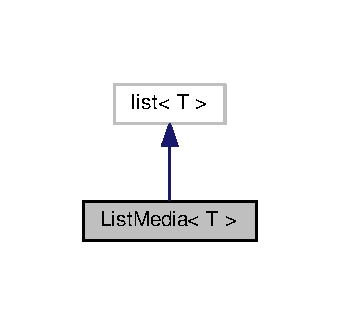
\includegraphics[width=163pt]{classListMedia__inherit__graph}
\end{center}
\end{figure}


Collaboration diagram for List\+Media$<$ T $>$\+:
\nopagebreak
\begin{figure}[H]
\begin{center}
\leavevmode
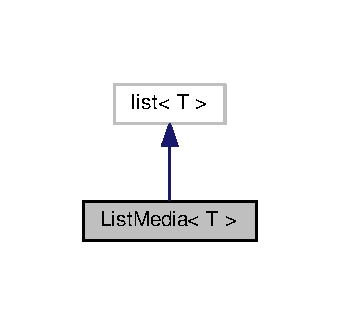
\includegraphics[width=163pt]{classListMedia__coll__graph}
\end{center}
\end{figure}
\subsection*{Public Member Functions}
\begin{DoxyCompactItemize}
\item 
\hypertarget{classListMedia_aabaa65f0e12e2448929cdbf186c460a1}{{\bfseries List\+Media} (string \+\_\+name=\char`\"{}\char`\"{})}\label{classListMedia_aabaa65f0e12e2448929cdbf186c460a1}

\item 
virtual string \hyperlink{classListMedia_a47a421d3239b06ffd124fc9c8975f052}{getname} () const 
\begin{DoxyCompactList}\small\item\em getname \end{DoxyCompactList}\item 
virtual void \hyperlink{classListMedia_a72299db4f3ae463da585fc943387320c}{display} (ostream \&out, bool flag=false) const 
\begin{DoxyCompactList}\small\item\em display \end{DoxyCompactList}\end{DoxyCompactItemize}


\subsection{Member Function Documentation}
\hypertarget{classListMedia_a72299db4f3ae463da585fc943387320c}{\index{List\+Media@{List\+Media}!display@{display}}
\index{display@{display}!List\+Media@{List\+Media}}
\subsubsection[{display}]{\setlength{\rightskip}{0pt plus 5cm}template$<$typename T $>$ virtual void {\bf List\+Media}$<$ T $>$\+::display (
\begin{DoxyParamCaption}
\item[{ostream \&}]{out, }
\item[{bool}]{flag = {\ttfamily false}}
\end{DoxyParamCaption}
) const\hspace{0.3cm}{\ttfamily [inline]}, {\ttfamily [virtual]}}}\label{classListMedia_a72299db4f3ae463da585fc943387320c}


display 


\begin{DoxyParams}{Parameters}
{\em out,flag} & \\
\hline
\end{DoxyParams}
\begin{DoxyReturn}{Returns}
show the information of the media in the list flag is to judge if it is used for cout or server 
\end{DoxyReturn}
\hypertarget{classListMedia_a47a421d3239b06ffd124fc9c8975f052}{\index{List\+Media@{List\+Media}!getname@{getname}}
\index{getname@{getname}!List\+Media@{List\+Media}}
\subsubsection[{getname}]{\setlength{\rightskip}{0pt plus 5cm}template$<$typename T $>$ virtual string {\bf List\+Media}$<$ T $>$\+::getname (
\begin{DoxyParamCaption}
{}
\end{DoxyParamCaption}
) const\hspace{0.3cm}{\ttfamily [inline]}, {\ttfamily [virtual]}}}\label{classListMedia_a47a421d3239b06ffd124fc9c8975f052}


getname 


\begin{DoxyParams}{Parameters}
{\em } & return name\+\_\+group  get the name of group \\
\hline
\end{DoxyParams}


The documentation for this class was generated from the following file\+:\begin{DoxyCompactItemize}
\item 
listmedia.\+h\end{DoxyCompactItemize}

\hypertarget{classMultimedia}{\section{Multimedia Class Reference}
\label{classMultimedia}\index{Multimedia@{Multimedia}}
}


Inheritance diagram for Multimedia\+:
\nopagebreak
\begin{figure}[H]
\begin{center}
\leavevmode
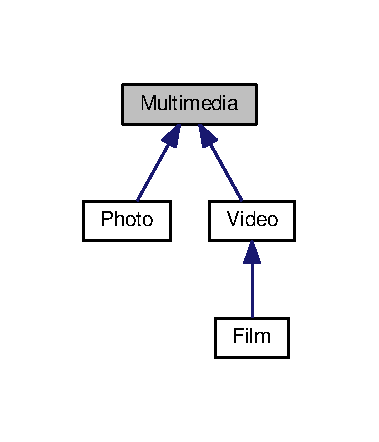
\includegraphics[width=182pt]{classMultimedia__inherit__graph}
\end{center}
\end{figure}
\subsection*{Public Member Functions}
\begin{DoxyCompactItemize}
\item 
\hyperlink{classMultimedia_a7106753d618df92d53b89328b7ecfe7f}{Multimedia} ()
\begin{DoxyCompactList}\small\item\em \hyperlink{classMultimedia}{Multimedia}. \end{DoxyCompactList}\item 
\hyperlink{classMultimedia_a3f8beee15410ad6bbf9fa6caf0599a61}{Multimedia} (string \+\_\+nom\+F, string \+\_\+nom\+M, string \+\_\+nom\+C)
\begin{DoxyCompactList}\small\item\em \hyperlink{classMultimedia}{Multimedia}. \end{DoxyCompactList}\item 
virtual \hyperlink{classMultimedia_ab280f9ce1d0a1291c9b1ab876e854c94}{$\sim$\+Multimedia} ()
\begin{DoxyCompactList}\small\item\em $\sim$\+Multimedia \end{DoxyCompactList}\item 
virtual string \hyperlink{classMultimedia_a64cbf598c8500661be01792af535525c}{getnom\+F} () const 
\begin{DoxyCompactList}\small\item\em getnom\+F \end{DoxyCompactList}\item 
virtual void \hyperlink{classMultimedia_abc834ac0f75cf8d899912c3f72d289e0}{setnom\+F} (string \+\_\+nom\+F)
\begin{DoxyCompactList}\small\item\em setnom\+F \end{DoxyCompactList}\item 
virtual string \hyperlink{classMultimedia_a5e3458ee12aaf2b873f6ce0751c6e6a7}{getnom\+M} () const 
\begin{DoxyCompactList}\small\item\em getnom\+M \end{DoxyCompactList}\item 
virtual void \hyperlink{classMultimedia_ad06cc11ab564dcf2e819bdcca03e9439}{setnom\+M} (string \+\_\+nom\+M)
\begin{DoxyCompactList}\small\item\em setnom\+M \end{DoxyCompactList}\item 
virtual void \hyperlink{classMultimedia_a47176f027bfb92e5374cf34f4c70809a}{display} (ostream \&out, bool flag=false)
\begin{DoxyCompactList}\small\item\em display \end{DoxyCompactList}\item 
virtual void \hyperlink{classMultimedia_ad08d517e03460d941915682e8d0a13be}{play} () const =0
\begin{DoxyCompactList}\small\item\em play \end{DoxyCompactList}\item 
virtual string \hyperlink{classMultimedia_a76f1f1c9bd8fc12aecc145105b413898}{get\+Class\+Media} () const 
\begin{DoxyCompactList}\small\item\em get\+Class\+Media \end{DoxyCompactList}\end{DoxyCompactItemize}
\subsection*{Protected Attributes}
\begin{DoxyCompactItemize}
\item 
\hypertarget{classMultimedia_aa960228dfddde725c66d89d79e8fab43}{string {\bfseries class\+Media} = \char`\"{}\char`\"{}}\label{classMultimedia_aa960228dfddde725c66d89d79e8fab43}

\end{DoxyCompactItemize}


\subsection{Constructor \& Destructor Documentation}
\hypertarget{classMultimedia_a7106753d618df92d53b89328b7ecfe7f}{\index{Multimedia@{Multimedia}!Multimedia@{Multimedia}}
\index{Multimedia@{Multimedia}!Multimedia@{Multimedia}}
\subsubsection[{Multimedia}]{\setlength{\rightskip}{0pt plus 5cm}Multimedia\+::\+Multimedia (
\begin{DoxyParamCaption}
{}
\end{DoxyParamCaption}
)}}\label{classMultimedia_a7106753d618df92d53b89328b7ecfe7f}


\hyperlink{classMultimedia}{Multimedia}. 


\begin{DoxyParams}{Parameters}
{\em } & return  initializer nom\+Fichier, nom\+Media without parameter \\
\hline
\end{DoxyParams}
\hypertarget{classMultimedia_a3f8beee15410ad6bbf9fa6caf0599a61}{\index{Multimedia@{Multimedia}!Multimedia@{Multimedia}}
\index{Multimedia@{Multimedia}!Multimedia@{Multimedia}}
\subsubsection[{Multimedia}]{\setlength{\rightskip}{0pt plus 5cm}Multimedia\+::\+Multimedia (
\begin{DoxyParamCaption}
\item[{string}]{\+\_\+nom\+F, }
\item[{string}]{\+\_\+nom\+M, }
\item[{string}]{\+\_\+nom\+C}
\end{DoxyParamCaption}
)}}\label{classMultimedia_a3f8beee15410ad6bbf9fa6caf0599a61}


\hyperlink{classMultimedia}{Multimedia}. 


\begin{DoxyParams}{Parameters}
{\em } & return  initializer nom\+Fichier, nom\+Media with parameter \\
\hline
\end{DoxyParams}
\hypertarget{classMultimedia_ab280f9ce1d0a1291c9b1ab876e854c94}{\index{Multimedia@{Multimedia}!````~Multimedia@{$\sim$\+Multimedia}}
\index{````~Multimedia@{$\sim$\+Multimedia}!Multimedia@{Multimedia}}
\subsubsection[{$\sim$\+Multimedia}]{\setlength{\rightskip}{0pt plus 5cm}Multimedia\+::$\sim$\+Multimedia (
\begin{DoxyParamCaption}
{}
\end{DoxyParamCaption}
)\hspace{0.3cm}{\ttfamily [virtual]}}}\label{classMultimedia_ab280f9ce1d0a1291c9b1ab876e854c94}


$\sim$\+Multimedia 


\begin{DoxyParams}{Parameters}
{\em } & return  Output the information of destruction \\
\hline
\end{DoxyParams}


\subsection{Member Function Documentation}
\hypertarget{classMultimedia_a47176f027bfb92e5374cf34f4c70809a}{\index{Multimedia@{Multimedia}!display@{display}}
\index{display@{display}!Multimedia@{Multimedia}}
\subsubsection[{display}]{\setlength{\rightskip}{0pt plus 5cm}void Multimedia\+::display (
\begin{DoxyParamCaption}
\item[{ostream \&}]{out, }
\item[{bool}]{flag = {\ttfamily false}}
\end{DoxyParamCaption}
)\hspace{0.3cm}{\ttfamily [virtual]}}}\label{classMultimedia_a47176f027bfb92e5374cf34f4c70809a}


display 


\begin{DoxyParams}{Parameters}
{\em } & return  show the information of the multimedia \\
\hline
\end{DoxyParams}


Reimplemented in \hyperlink{classPhoto_a7a6e076a522a19422459af9e7f3c958b}{Photo}, \hyperlink{classVideo_a2f1902c8131fc232926e34487b54e0b9}{Video}, and \hyperlink{classFilm_a9f6a67ac8aa1e16501676c70e35d4eb4}{Film}.

\hypertarget{classMultimedia_a76f1f1c9bd8fc12aecc145105b413898}{\index{Multimedia@{Multimedia}!get\+Class\+Media@{get\+Class\+Media}}
\index{get\+Class\+Media@{get\+Class\+Media}!Multimedia@{Multimedia}}
\subsubsection[{get\+Class\+Media}]{\setlength{\rightskip}{0pt plus 5cm}string Multimedia\+::get\+Class\+Media (
\begin{DoxyParamCaption}
{}
\end{DoxyParamCaption}
) const\hspace{0.3cm}{\ttfamily [virtual]}}}\label{classMultimedia_a76f1f1c9bd8fc12aecc145105b413898}


get\+Class\+Media 


\begin{DoxyParams}{Parameters}
{\em } & return class\+Media  return class\+Media \\
\hline
\end{DoxyParams}
\hypertarget{classMultimedia_a64cbf598c8500661be01792af535525c}{\index{Multimedia@{Multimedia}!getnom\+F@{getnom\+F}}
\index{getnom\+F@{getnom\+F}!Multimedia@{Multimedia}}
\subsubsection[{getnom\+F}]{\setlength{\rightskip}{0pt plus 5cm}string Multimedia\+::getnom\+F (
\begin{DoxyParamCaption}
{}
\end{DoxyParamCaption}
) const\hspace{0.3cm}{\ttfamily [virtual]}}}\label{classMultimedia_a64cbf598c8500661be01792af535525c}


getnom\+F 


\begin{DoxyParams}{Parameters}
{\em } & return nom\+Fichier  return nom\+Fichier \\
\hline
\end{DoxyParams}
\hypertarget{classMultimedia_a5e3458ee12aaf2b873f6ce0751c6e6a7}{\index{Multimedia@{Multimedia}!getnom\+M@{getnom\+M}}
\index{getnom\+M@{getnom\+M}!Multimedia@{Multimedia}}
\subsubsection[{getnom\+M}]{\setlength{\rightskip}{0pt plus 5cm}string Multimedia\+::getnom\+M (
\begin{DoxyParamCaption}
{}
\end{DoxyParamCaption}
) const\hspace{0.3cm}{\ttfamily [virtual]}}}\label{classMultimedia_a5e3458ee12aaf2b873f6ce0751c6e6a7}


getnom\+M 


\begin{DoxyParams}{Parameters}
{\em } & return getnom\+M  return nom\+Media \\
\hline
\end{DoxyParams}
\hypertarget{classMultimedia_ad08d517e03460d941915682e8d0a13be}{\index{Multimedia@{Multimedia}!play@{play}}
\index{play@{play}!Multimedia@{Multimedia}}
\subsubsection[{play}]{\setlength{\rightskip}{0pt plus 5cm}void Multimedia\+::play (
\begin{DoxyParamCaption}
{}
\end{DoxyParamCaption}
) const\hspace{0.3cm}{\ttfamily [pure virtual]}}}\label{classMultimedia_ad08d517e03460d941915682e8d0a13be}


play 


\begin{DoxyParams}{Parameters}
{\em } & return  \\
\hline
\end{DoxyParams}


Implemented in \hyperlink{classPhoto_a34ef1c73e123d2951e8a08b3b1697c05}{Photo}, and \hyperlink{classVideo_acb8fdb5186d3b35672b9218375cf4f0b}{Video}.

\hypertarget{classMultimedia_abc834ac0f75cf8d899912c3f72d289e0}{\index{Multimedia@{Multimedia}!setnom\+F@{setnom\+F}}
\index{setnom\+F@{setnom\+F}!Multimedia@{Multimedia}}
\subsubsection[{setnom\+F}]{\setlength{\rightskip}{0pt plus 5cm}void Multimedia\+::setnom\+F (
\begin{DoxyParamCaption}
\item[{string}]{\+\_\+nom\+F}
\end{DoxyParamCaption}
)\hspace{0.3cm}{\ttfamily [virtual]}}}\label{classMultimedia_abc834ac0f75cf8d899912c3f72d289e0}


setnom\+F 


\begin{DoxyParams}{Parameters}
{\em \+\_\+nom\+F} & \\
\hline
\end{DoxyParams}
\begin{DoxyReturn}{Returns}
set the value of nom\+Fichier 
\end{DoxyReturn}
\hypertarget{classMultimedia_ad06cc11ab564dcf2e819bdcca03e9439}{\index{Multimedia@{Multimedia}!setnom\+M@{setnom\+M}}
\index{setnom\+M@{setnom\+M}!Multimedia@{Multimedia}}
\subsubsection[{setnom\+M}]{\setlength{\rightskip}{0pt plus 5cm}void Multimedia\+::setnom\+M (
\begin{DoxyParamCaption}
\item[{string}]{\+\_\+nom\+M}
\end{DoxyParamCaption}
)\hspace{0.3cm}{\ttfamily [virtual]}}}\label{classMultimedia_ad06cc11ab564dcf2e819bdcca03e9439}


setnom\+M 


\begin{DoxyParams}{Parameters}
{\em \+\_\+nom\+M} & \\
\hline
\end{DoxyParams}
\begin{DoxyReturn}{Returns}
et the value of nom\+Media 
\end{DoxyReturn}


The documentation for this class was generated from the following files\+:\begin{DoxyCompactItemize}
\item 
multimedia.\+h\item 
multimedia.\+cpp\end{DoxyCompactItemize}

\hypertarget{classMyBase}{\section{My\+Base Class Reference}
\label{classMyBase}\index{My\+Base@{My\+Base}}
}
\subsection*{Public Member Functions}
\begin{DoxyCompactItemize}
\item 
bool \hyperlink{classMyBase_a818864f09718a0aa6d65f5ac5733b689}{process\+Request} (\hyperlink{classcppu_1_1TCPConnection}{T\+C\+P\+Connection} \&cnx, const string \&request, string \&response)
\begin{DoxyCompactList}\small\item\em process\+Request \end{DoxyCompactList}\end{DoxyCompactItemize}


\subsection{Member Function Documentation}
\hypertarget{classMyBase_a818864f09718a0aa6d65f5ac5733b689}{\index{My\+Base@{My\+Base}!process\+Request@{process\+Request}}
\index{process\+Request@{process\+Request}!My\+Base@{My\+Base}}
\subsubsection[{process\+Request}]{\setlength{\rightskip}{0pt plus 5cm}bool My\+Base\+::process\+Request (
\begin{DoxyParamCaption}
\item[{{\bf T\+C\+P\+Connection} \&}]{cnx, }
\item[{const string \&}]{request, }
\item[{string \&}]{response}
\end{DoxyParamCaption}
)\hspace{0.3cm}{\ttfamily [inline]}}}\label{classMyBase_a818864f09718a0aa6d65f5ac5733b689}


process\+Request 


\begin{DoxyParams}{Parameters}
{\em cnx,request,response} & \\
\hline
\end{DoxyParams}
\begin{DoxyReturn}{Returns}
Process the request and give the right response according to the command For example, \char`\"{}create\+Photo;./;test.\+jpg;100;200\char`\"{} 
\end{DoxyReturn}


The documentation for this class was generated from the following file\+:\begin{DoxyCompactItemize}
\item 
server.\+cpp\end{DoxyCompactItemize}

\hypertarget{classPhoto}{\section{Photo Class Reference}
\label{classPhoto}\index{Photo@{Photo}}
}


Inheritance diagram for Photo\+:
\nopagebreak
\begin{figure}[H]
\begin{center}
\leavevmode
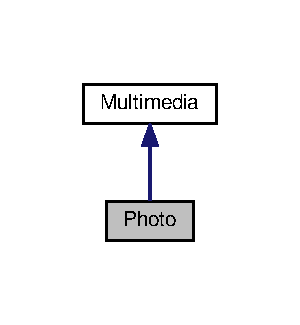
\includegraphics[width=144pt]{classPhoto__inherit__graph}
\end{center}
\end{figure}


Collaboration diagram for Photo\+:
\nopagebreak
\begin{figure}[H]
\begin{center}
\leavevmode
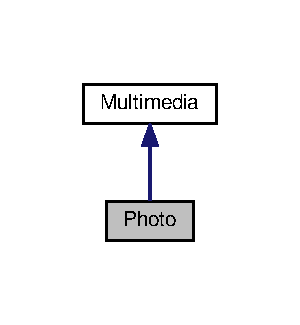
\includegraphics[width=144pt]{classPhoto__coll__graph}
\end{center}
\end{figure}
\subsection*{Public Member Functions}
\begin{DoxyCompactItemize}
\item 
\hyperlink{classPhoto_ac927f9690ec0d6901371ea8171f45853}{Photo} (string \+\_\+nom\+F=\char`\"{}\char`\"{}, string \+\_\+nom\+M=\char`\"{}\char`\"{}, double \+\_\+latitude=0, double \+\_\+longitude=0)
\begin{DoxyCompactList}\small\item\em \hyperlink{classMultimedia}{Multimedia}. \end{DoxyCompactList}\item 
virtual double \hyperlink{classPhoto_a75f9548586cedcbb6639bc74f7559a46}{get\+Latitude} () const 
\begin{DoxyCompactList}\small\item\em get\+Latitude \end{DoxyCompactList}\item 
virtual void \hyperlink{classPhoto_abf629ddab24eb9e5c887ea75b1a283a9}{set\+Latitude} (double \+\_\+latitude)
\begin{DoxyCompactList}\small\item\em set\+Latitude \end{DoxyCompactList}\item 
virtual double \hyperlink{classPhoto_a6e2def6e43b3dd8eee78fcafe34dcaff}{get\+Longitude} () const 
\begin{DoxyCompactList}\small\item\em get\+Longitude \end{DoxyCompactList}\item 
virtual void \hyperlink{classPhoto_a1352b8982d0f72a82abb3f69d798ea01}{set\+Longitude} (double \+\_\+longitude)
\begin{DoxyCompactList}\small\item\em set\+Longitude \end{DoxyCompactList}\item 
virtual void \hyperlink{classPhoto_a7a6e076a522a19422459af9e7f3c958b}{display} (ostream \&out, bool flag=false)
\begin{DoxyCompactList}\small\item\em display \end{DoxyCompactList}\item 
virtual void \hyperlink{classPhoto_a34ef1c73e123d2951e8a08b3b1697c05}{play} () const 
\begin{DoxyCompactList}\small\item\em play \end{DoxyCompactList}\end{DoxyCompactItemize}
\subsection*{Additional Inherited Members}


\subsection{Constructor \& Destructor Documentation}
\hypertarget{classPhoto_ac927f9690ec0d6901371ea8171f45853}{\index{Photo@{Photo}!Photo@{Photo}}
\index{Photo@{Photo}!Photo@{Photo}}
\subsubsection[{Photo}]{\setlength{\rightskip}{0pt plus 5cm}Photo\+::\+Photo (
\begin{DoxyParamCaption}
\item[{string}]{\+\_\+nom\+F = {\ttfamily \char`\"{}\char`\"{}}, }
\item[{string}]{\+\_\+nom\+M = {\ttfamily \char`\"{}\char`\"{}}, }
\item[{double}]{\+\_\+latitude = {\ttfamily 0}, }
\item[{double}]{\+\_\+longitude = {\ttfamily 0}}
\end{DoxyParamCaption}
)}}\label{classPhoto_ac927f9690ec0d6901371ea8171f45853}


\hyperlink{classMultimedia}{Multimedia}. 


\begin{DoxyParams}{Parameters}
{\em } & return  initializer nom\+Fichier, nom\+Media with parameter and inherit the constructer of multimedia \\
\hline
\end{DoxyParams}


\subsection{Member Function Documentation}
\hypertarget{classPhoto_a7a6e076a522a19422459af9e7f3c958b}{\index{Photo@{Photo}!display@{display}}
\index{display@{display}!Photo@{Photo}}
\subsubsection[{display}]{\setlength{\rightskip}{0pt plus 5cm}void Photo\+::display (
\begin{DoxyParamCaption}
\item[{ostream \&}]{out, }
\item[{bool}]{flag = {\ttfamily false}}
\end{DoxyParamCaption}
)\hspace{0.3cm}{\ttfamily [virtual]}}}\label{classPhoto_a7a6e076a522a19422459af9e7f3c958b}


display 


\begin{DoxyParams}{Parameters}
{\em out,flag} & \\
\hline
\end{DoxyParams}
\begin{DoxyReturn}{Returns}
show the information of the photo, flag is to judge if it is used for cout or server 
\end{DoxyReturn}


Reimplemented from \hyperlink{classMultimedia_a47176f027bfb92e5374cf34f4c70809a}{Multimedia}.

\hypertarget{classPhoto_a75f9548586cedcbb6639bc74f7559a46}{\index{Photo@{Photo}!get\+Latitude@{get\+Latitude}}
\index{get\+Latitude@{get\+Latitude}!Photo@{Photo}}
\subsubsection[{get\+Latitude}]{\setlength{\rightskip}{0pt plus 5cm}double Photo\+::get\+Latitude (
\begin{DoxyParamCaption}
{}
\end{DoxyParamCaption}
) const\hspace{0.3cm}{\ttfamily [virtual]}}}\label{classPhoto_a75f9548586cedcbb6639bc74f7559a46}


get\+Latitude 


\begin{DoxyParams}{Parameters}
{\em } & return latitude  get the value of latitude \\
\hline
\end{DoxyParams}
\hypertarget{classPhoto_a6e2def6e43b3dd8eee78fcafe34dcaff}{\index{Photo@{Photo}!get\+Longitude@{get\+Longitude}}
\index{get\+Longitude@{get\+Longitude}!Photo@{Photo}}
\subsubsection[{get\+Longitude}]{\setlength{\rightskip}{0pt plus 5cm}double Photo\+::get\+Longitude (
\begin{DoxyParamCaption}
{}
\end{DoxyParamCaption}
) const\hspace{0.3cm}{\ttfamily [virtual]}}}\label{classPhoto_a6e2def6e43b3dd8eee78fcafe34dcaff}


get\+Longitude 


\begin{DoxyParams}{Parameters}
{\em } & return longitude  get the value of longitude \\
\hline
\end{DoxyParams}
\hypertarget{classPhoto_a34ef1c73e123d2951e8a08b3b1697c05}{\index{Photo@{Photo}!play@{play}}
\index{play@{play}!Photo@{Photo}}
\subsubsection[{play}]{\setlength{\rightskip}{0pt plus 5cm}void Photo\+::play (
\begin{DoxyParamCaption}
{}
\end{DoxyParamCaption}
) const\hspace{0.3cm}{\ttfamily [virtual]}}}\label{classPhoto_a34ef1c73e123d2951e8a08b3b1697c05}


play 


\begin{DoxyParams}{Parameters}
{\em } & return  show the photo \\
\hline
\end{DoxyParams}


Implements \hyperlink{classMultimedia_ad08d517e03460d941915682e8d0a13be}{Multimedia}.

\hypertarget{classPhoto_abf629ddab24eb9e5c887ea75b1a283a9}{\index{Photo@{Photo}!set\+Latitude@{set\+Latitude}}
\index{set\+Latitude@{set\+Latitude}!Photo@{Photo}}
\subsubsection[{set\+Latitude}]{\setlength{\rightskip}{0pt plus 5cm}void Photo\+::set\+Latitude (
\begin{DoxyParamCaption}
\item[{double}]{\+\_\+latitude}
\end{DoxyParamCaption}
)\hspace{0.3cm}{\ttfamily [virtual]}}}\label{classPhoto_abf629ddab24eb9e5c887ea75b1a283a9}


set\+Latitude 


\begin{DoxyParams}{Parameters}
{\em \+\_\+latitude} & \\
\hline
\end{DoxyParams}
\begin{DoxyReturn}{Returns}
set the value of latitude 
\end{DoxyReturn}
\hypertarget{classPhoto_a1352b8982d0f72a82abb3f69d798ea01}{\index{Photo@{Photo}!set\+Longitude@{set\+Longitude}}
\index{set\+Longitude@{set\+Longitude}!Photo@{Photo}}
\subsubsection[{set\+Longitude}]{\setlength{\rightskip}{0pt plus 5cm}void Photo\+::set\+Longitude (
\begin{DoxyParamCaption}
\item[{double}]{\+\_\+longitude}
\end{DoxyParamCaption}
)\hspace{0.3cm}{\ttfamily [virtual]}}}\label{classPhoto_a1352b8982d0f72a82abb3f69d798ea01}


set\+Longitude 


\begin{DoxyParams}{Parameters}
{\em \+\_\+longitude} & \\
\hline
\end{DoxyParams}
\begin{DoxyReturn}{Returns}
set the value of longitude 
\end{DoxyReturn}


The documentation for this class was generated from the following files\+:\begin{DoxyCompactItemize}
\item 
photo.\+h\item 
photo.\+cpp\end{DoxyCompactItemize}

\hypertarget{classcppu_1_1ServerSocket}{\section{cppu\+:\+:Server\+Socket Class Reference}
\label{classcppu_1_1ServerSocket}\index{cppu\+::\+Server\+Socket@{cppu\+::\+Server\+Socket}}
}


T\+C\+P/\+I\+P server socket. This class implements a T\+C\+P/\+I\+P socket that waits for requests to come in over the network. A\+F\+\_\+\+I\+N\+E\+T connections following the I\+Pv4 Internet protocol are supported.  




{\ttfamily \#include $<$cppsocket.\+h$>$}

\subsection*{Public Member Functions}
\begin{DoxyCompactItemize}
\item 
\hypertarget{classcppu_1_1ServerSocket_a57138f5a7d2e8af35228c8985385c494}{\hyperlink{classcppu_1_1ServerSocket_a57138f5a7d2e8af35228c8985385c494}{Server\+Socket} ()}\label{classcppu_1_1ServerSocket_a57138f5a7d2e8af35228c8985385c494}

\begin{DoxyCompactList}\small\item\em Creates a new server socket. Creates a listening socket that waits for connection requests by T\+C\+P/\+I\+P clients. \end{DoxyCompactList}\item 
virtual \hyperlink{classcppu_1_1Socket}{Socket} $\ast$ \hyperlink{classcppu_1_1ServerSocket_af08ebcb886fc778d195fb622f7b96b8b}{accept} ()
\begin{DoxyCompactList}\small\item\em Accepts a new connection request and returns the corresponding socket. By default, this function blocks the caller until a connection is present. \end{DoxyCompactList}\item 
virtual int \hyperlink{classcppu_1_1ServerSocket_a255dfdccba51c7cdbcb6733c6c3f6ffa}{bind} (int port, int backlog=50)
\begin{DoxyCompactList}\small\item\em Assigns the socket to the local address. The socket must be bound before using it. \end{DoxyCompactList}\item 
\hypertarget{classcppu_1_1ServerSocket_ae7647cfb5beaf504a846f6ecfdd197c4}{virtual int \hyperlink{classcppu_1_1ServerSocket_ae7647cfb5beaf504a846f6ecfdd197c4}{close} ()}\label{classcppu_1_1ServerSocket_ae7647cfb5beaf504a846f6ecfdd197c4}

\begin{DoxyCompactList}\small\item\em Closes the socket. \end{DoxyCompactList}\item 
\hypertarget{classcppu_1_1ServerSocket_aa3ca8fed354955eeb45af3a2021c04cb}{bool \hyperlink{classcppu_1_1ServerSocket_aa3ca8fed354955eeb45af3a2021c04cb}{is\+Closed} () const }\label{classcppu_1_1ServerSocket_aa3ca8fed354955eeb45af3a2021c04cb}

\begin{DoxyCompactList}\small\item\em Returns true if the socket has been closed. \end{DoxyCompactList}\item 
\hypertarget{classcppu_1_1ServerSocket_a905d85f63fdca46ed5ee44eb00e211d1}{int \hyperlink{classcppu_1_1ServerSocket_a905d85f63fdca46ed5ee44eb00e211d1}{descriptor} ()}\label{classcppu_1_1ServerSocket_a905d85f63fdca46ed5ee44eb00e211d1}

\begin{DoxyCompactList}\small\item\em Returns the Unix descriptor of the socket. \end{DoxyCompactList}\item 
\hypertarget{classcppu_1_1ServerSocket_a0fbd0ee42bcfecf2e749279c4b94b0b3}{int \hyperlink{classcppu_1_1ServerSocket_a0fbd0ee42bcfecf2e749279c4b94b0b3}{set\+Receive\+Buffer\+Size} (int size)}\label{classcppu_1_1ServerSocket_a0fbd0ee42bcfecf2e749279c4b94b0b3}

\begin{DoxyCompactList}\small\item\em Sets the S\+O\+\_\+\+R\+C\+V\+B\+U\+F option to the specified value. \end{DoxyCompactList}\item 
\hypertarget{classcppu_1_1ServerSocket_a09d0494cc0f65abe496b9c940d2920ed}{int \hyperlink{classcppu_1_1ServerSocket_a09d0494cc0f65abe496b9c940d2920ed}{set\+Reuse\+Address} (bool)}\label{classcppu_1_1ServerSocket_a09d0494cc0f65abe496b9c940d2920ed}

\begin{DoxyCompactList}\small\item\em Enables/disables the S\+O\+\_\+\+R\+E\+U\+S\+E\+A\+D\+D\+R socket option. \end{DoxyCompactList}\item 
\hypertarget{classcppu_1_1ServerSocket_a0ceb984eab0cdd9c7c8e62658a521175}{int \hyperlink{classcppu_1_1ServerSocket_a0ceb984eab0cdd9c7c8e62658a521175}{set\+So\+Timeout} (int timeout)}\label{classcppu_1_1ServerSocket_a0ceb984eab0cdd9c7c8e62658a521175}

\begin{DoxyCompactList}\small\item\em Enables/disables S\+O\+\_\+\+T\+I\+M\+E\+O\+U\+T with the specified timeout (in milliseconds). \end{DoxyCompactList}\item 
\hypertarget{classcppu_1_1ServerSocket_ac5f6da333208cce9ca4d5392259a0a6b}{int \hyperlink{classcppu_1_1ServerSocket_ac5f6da333208cce9ca4d5392259a0a6b}{set\+Tcp\+No\+Delay} (bool)}\label{classcppu_1_1ServerSocket_ac5f6da333208cce9ca4d5392259a0a6b}

\begin{DoxyCompactList}\small\item\em Turns on/off T\+C\+P coalescence (useful in some cases to avoid delays). \end{DoxyCompactList}\end{DoxyCompactItemize}
\subsection*{Protected Member Functions}
\begin{DoxyCompactItemize}
\item 
\hypertarget{classcppu_1_1ServerSocket_a23d038275576d0a969072eb334f7b84f}{virtual \hyperlink{classcppu_1_1Socket}{Socket} $\ast$ {\bfseries create\+Socket} (int sockfd)}\label{classcppu_1_1ServerSocket_a23d038275576d0a969072eb334f7b84f}

\end{DoxyCompactItemize}


\subsection{Detailed Description}
T\+C\+P/\+I\+P server socket. This class implements a T\+C\+P/\+I\+P socket that waits for requests to come in over the network. A\+F\+\_\+\+I\+N\+E\+T connections following the I\+Pv4 Internet protocol are supported. 

\begin{DoxyNote}{Note}
T\+C\+P/\+I\+P sockets do not preserve record boundaries, 
\end{DoxyNote}
\begin{DoxySeeAlso}{See also}
\hyperlink{classcppu_1_1SocketBuffer}{Socket\+Buffer} for a solution. 
\end{DoxySeeAlso}


\subsection{Member Function Documentation}
\hypertarget{classcppu_1_1ServerSocket_af08ebcb886fc778d195fb622f7b96b8b}{\index{cppu\+::\+Server\+Socket@{cppu\+::\+Server\+Socket}!accept@{accept}}
\index{accept@{accept}!cppu\+::\+Server\+Socket@{cppu\+::\+Server\+Socket}}
\subsubsection[{accept}]{\setlength{\rightskip}{0pt plus 5cm}{\bf Socket} $\ast$ cppu\+::\+Server\+Socket\+::accept (
\begin{DoxyParamCaption}
{}
\end{DoxyParamCaption}
)\hspace{0.3cm}{\ttfamily [virtual]}}}\label{classcppu_1_1ServerSocket_af08ebcb886fc778d195fb622f7b96b8b}


Accepts a new connection request and returns the corresponding socket. By default, this function blocks the caller until a connection is present. 

\begin{DoxyReturn}{Returns}
the new \hyperlink{classcppu_1_1Socket}{Socket} or nullptr on error. 
\end{DoxyReturn}
\hypertarget{classcppu_1_1ServerSocket_a255dfdccba51c7cdbcb6733c6c3f6ffa}{\index{cppu\+::\+Server\+Socket@{cppu\+::\+Server\+Socket}!bind@{bind}}
\index{bind@{bind}!cppu\+::\+Server\+Socket@{cppu\+::\+Server\+Socket}}
\subsubsection[{bind}]{\setlength{\rightskip}{0pt plus 5cm}int cppu\+::\+Server\+Socket\+::bind (
\begin{DoxyParamCaption}
\item[{int}]{port, }
\item[{int}]{backlog = {\ttfamily 50}}
\end{DoxyParamCaption}
)\hspace{0.3cm}{\ttfamily [virtual]}}}\label{classcppu_1_1ServerSocket_a255dfdccba51c7cdbcb6733c6c3f6ffa}


Assigns the socket to the local address. The socket must be bound before using it. 

\begin{DoxyReturn}{Returns}
0 on success or a negative value on error which is one of \hyperlink{classcppu_1_1Socket_a49ea5cb079bd7ae97ecf7eb30c9d9e5f}{Socket\+::\+Errors} 
\end{DoxyReturn}


The documentation for this class was generated from the following files\+:\begin{DoxyCompactItemize}
\item 
cppsocket.\+h\item 
cppsocket.\+cpp\end{DoxyCompactItemize}

\hypertarget{classcppu_1_1Socket}{\section{cppu\+:\+:Socket Class Reference}
\label{classcppu_1_1Socket}\index{cppu\+::\+Socket@{cppu\+::\+Socket}}
}


T\+C\+P/\+I\+P or U\+D\+P/\+Datagram socket. This class encapsulates a T\+C\+P/\+I\+P or U\+D\+P/\+Datagram socket. A\+F\+\_\+\+I\+N\+E\+T connections following the I\+Pv4 Internet protocol are supported.  




{\ttfamily \#include $<$cppsocket.\+h$>$}

\subsection*{Public Types}
\begin{DoxyCompactItemize}
\item 
enum \hyperlink{classcppu_1_1Socket_a49ea5cb079bd7ae97ecf7eb30c9d9e5f}{Errors} \{ {\bfseries Failed} = -\/1, 
{\bfseries Invalid\+Socket} = -\/2, 
{\bfseries Unknown\+Host} = -\/3
 \}
\begin{DoxyCompactList}\small\item\em \hyperlink{classcppu_1_1Socket}{Socket} errors. \end{DoxyCompactList}\end{DoxyCompactItemize}
\subsection*{Public Member Functions}
\begin{DoxyCompactItemize}
\item 
\hyperlink{classcppu_1_1Socket_ae73b9b629fe443f650203d938f61a279}{Socket} (int type=S\+O\+C\+K\+\_\+\+S\+T\+R\+E\+A\+M)
\begin{DoxyCompactList}\small\item\em Creates a new \hyperlink{classcppu_1_1Socket}{Socket}. Creates a A\+F\+\_\+\+I\+N\+E\+T socket using the I\+Pv4 Internet protocol. Type can be\+: \end{DoxyCompactList}\item 
\hypertarget{classcppu_1_1Socket_a8404e4e80cc625a4be32aacc879bb237}{\hyperlink{classcppu_1_1Socket_a8404e4e80cc625a4be32aacc879bb237}{Socket} (int type, int sockfd)}\label{classcppu_1_1Socket_a8404e4e80cc625a4be32aacc879bb237}

\begin{DoxyCompactList}\small\item\em Creates a \hyperlink{classcppu_1_1Socket}{Socket} object from an existing socket file descriptor. \end{DoxyCompactList}\item 
\hypertarget{classcppu_1_1Socket_ae26733a0b7d8a5fb5544d2d069152de7}{virtual \hyperlink{classcppu_1_1Socket_ae26733a0b7d8a5fb5544d2d069152de7}{$\sim$\+Socket} ()}\label{classcppu_1_1Socket_ae26733a0b7d8a5fb5544d2d069152de7}

\begin{DoxyCompactList}\small\item\em Destructor (closes the socket). \end{DoxyCompactList}\item 
virtual int \hyperlink{classcppu_1_1Socket_a7b876dcaff0babaffde41575f9b19d64}{bind} (int port)
\begin{DoxyCompactList}\small\item\em Assigns the socket to the local address. Typically used for U\+D\+P/\+Datagram sockets,. \end{DoxyCompactList}\item 
virtual int \hyperlink{classcppu_1_1Socket_a5698a3a7c6c203676c6de5e5559a0a7f}{bind} (const std\+::string \&host, int port)
\begin{DoxyCompactList}\small\item\em Assigns the socket to an address. Typically used for U\+D\+P/\+Datagram sockets,. \end{DoxyCompactList}\item 
virtual int \hyperlink{classcppu_1_1Socket_af6db3840caee709738f0e2a9ff814e5d}{connect} (const std\+::string \&host, int port)
\begin{DoxyCompactList}\small\item\em Connects the socket to an address. Typically used for T\+C\+P/\+I\+P sockets on the client side,. \end{DoxyCompactList}\item 
virtual int \hyperlink{classcppu_1_1Socket_ab958ef8a0f0495cf3a1c57a2ad4a34fc}{close} ()
\begin{DoxyCompactList}\small\item\em Closes the socket. \end{DoxyCompactList}\item 
\hypertarget{classcppu_1_1Socket_a726c2e6be413fe4e0584a23a173ae540}{bool \hyperlink{classcppu_1_1Socket_a726c2e6be413fe4e0584a23a173ae540}{is\+Closed} () const }\label{classcppu_1_1Socket_a726c2e6be413fe4e0584a23a173ae540}

\begin{DoxyCompactList}\small\item\em Returns true if the socket has been closed. \end{DoxyCompactList}\item 
\hypertarget{classcppu_1_1Socket_a06a8fcd9518e6a3e8b33bb64f7fb9036}{int \hyperlink{classcppu_1_1Socket_a06a8fcd9518e6a3e8b33bb64f7fb9036}{descriptor} ()}\label{classcppu_1_1Socket_a06a8fcd9518e6a3e8b33bb64f7fb9036}

\begin{DoxyCompactList}\small\item\em Returns the Unix descriptor of the socket. \end{DoxyCompactList}\item 
ssize\+\_\+t \hyperlink{classcppu_1_1Socket_aeac77f859159715e2d63a5a0dc118788}{send} (const void $\ast$buf, size\+\_\+t len, int flags=0)
\begin{DoxyCompactList}\small\item\em Sends data to a connected socket. Sends {\itshape len} bytes to a T\+C\+P/\+I\+P socket using the Unix \hyperlink{classcppu_1_1Socket_aeac77f859159715e2d63a5a0dc118788}{send()} function (. \end{DoxyCompactList}\item 
ssize\+\_\+t \hyperlink{classcppu_1_1Socket_a37c382af52cc02f92c0e19a0c6e0e04f}{receive} (void $\ast$buf, size\+\_\+t len, int flags=0)
\begin{DoxyCompactList}\small\item\em Receives data from a connected socket. Reads at most {\itshape len} bytes from a T\+C\+P/\+I\+P socket using the Unix recv() function. By default, this function blocks the caller until data is present (. \end{DoxyCompactList}\item 
ssize\+\_\+t \hyperlink{classcppu_1_1Socket_a31ff5137959aa4e52d4bcdd53e0b0069}{send\+To} (const void $\ast$buf, size\+\_\+t len, int flags, const struct sockaddr $\ast$dest\+\_\+addr, socklen\+\_\+t addrlen)
\begin{DoxyCompactList}\small\item\em Sends data to a datagram socket. Sends {\itshape len} bytes to a datagram socket using the Unix sendto() function. \end{DoxyCompactList}\item 
ssize\+\_\+t \hyperlink{classcppu_1_1Socket_abd460be82deeb29e730fc83f871e51c4}{receive\+From} (void $\ast$buf, size\+\_\+t len, int flags, struct sockaddr $\ast$src\+\_\+addr, socklen\+\_\+t $\ast$addrlen)
\begin{DoxyCompactList}\small\item\em Receives data from datagram socket. Reads at most {\itshape len} bytes from a datagram socket using the Unix recvfrom() function. By default, this function blocks the caller until data is present (. \end{DoxyCompactList}\item 
\hypertarget{classcppu_1_1Socket_a06c6838f267e5a0ba74558da946efb90}{virtual void \hyperlink{classcppu_1_1Socket_a06c6838f267e5a0ba74558da946efb90}{shutdown\+Input} ()}\label{classcppu_1_1Socket_a06c6838f267e5a0ba74558da946efb90}

\begin{DoxyCompactList}\small\item\em Disables further receive operations. \end{DoxyCompactList}\item 
\hypertarget{classcppu_1_1Socket_a97ee9ef3bf9fdecd6ae6f2b583b34d0e}{virtual void \hyperlink{classcppu_1_1Socket_a97ee9ef3bf9fdecd6ae6f2b583b34d0e}{shutdown\+Output} ()}\label{classcppu_1_1Socket_a97ee9ef3bf9fdecd6ae6f2b583b34d0e}

\begin{DoxyCompactList}\small\item\em Disables further send operations. \end{DoxyCompactList}\item 
\hypertarget{classcppu_1_1Socket_af172d5c78f63713988b0a6bf66851be7}{int \hyperlink{classcppu_1_1Socket_af172d5c78f63713988b0a6bf66851be7}{set\+Receive\+Buffer\+Size} (int size)}\label{classcppu_1_1Socket_af172d5c78f63713988b0a6bf66851be7}

\begin{DoxyCompactList}\small\item\em Sets the size of the T\+C\+P/\+I\+P input buffer. \end{DoxyCompactList}\item 
\hypertarget{classcppu_1_1Socket_a27b7fe34e172ad1f97c304d2786f624a}{int \hyperlink{classcppu_1_1Socket_a27b7fe34e172ad1f97c304d2786f624a}{set\+Reuse\+Address} (bool)}\label{classcppu_1_1Socket_a27b7fe34e172ad1f97c304d2786f624a}

\begin{DoxyCompactList}\small\item\em Enables/disables the S\+O\+\_\+\+R\+E\+U\+S\+E\+A\+D\+D\+R socket option. \end{DoxyCompactList}\item 
\hypertarget{classcppu_1_1Socket_aefda954454d860fa6a6d41b3d5cd26db}{int \hyperlink{classcppu_1_1Socket_aefda954454d860fa6a6d41b3d5cd26db}{set\+Send\+Buffer\+Size} (int size)}\label{classcppu_1_1Socket_aefda954454d860fa6a6d41b3d5cd26db}

\begin{DoxyCompactList}\small\item\em Sets the size of the T\+C\+P/\+I\+P output buffer. \end{DoxyCompactList}\item 
\hypertarget{classcppu_1_1Socket_ae87eb0335c072f765bf2b6a47162e7f5}{int \hyperlink{classcppu_1_1Socket_ae87eb0335c072f765bf2b6a47162e7f5}{set\+So\+Linger} (bool, int linger)}\label{classcppu_1_1Socket_ae87eb0335c072f765bf2b6a47162e7f5}

\begin{DoxyCompactList}\small\item\em Enables/disables S\+O\+\_\+\+L\+I\+N\+G\+E\+R with the specified linger time in seconds. \end{DoxyCompactList}\item 
\hypertarget{classcppu_1_1Socket_ae5dea30a1cae2dbdbdaf11a9f7ffa444}{int \hyperlink{classcppu_1_1Socket_ae5dea30a1cae2dbdbdaf11a9f7ffa444}{set\+So\+Timeout} (int timeout)}\label{classcppu_1_1Socket_ae5dea30a1cae2dbdbdaf11a9f7ffa444}

\begin{DoxyCompactList}\small\item\em Enables/disables S\+O\+\_\+\+T\+I\+M\+E\+O\+U\+T with the specified timeout (in milliseconds). \end{DoxyCompactList}\item 
\hypertarget{classcppu_1_1Socket_a6b29a9e12926b07f65b8dc52176131c5}{int \hyperlink{classcppu_1_1Socket_a6b29a9e12926b07f65b8dc52176131c5}{set\+Tcp\+No\+Delay} (bool)}\label{classcppu_1_1Socket_a6b29a9e12926b07f65b8dc52176131c5}

\begin{DoxyCompactList}\small\item\em Enables/disables T\+C\+P\+\_\+\+N\+O\+D\+E\+L\+A\+Y (turns on/off T\+C\+P coalescence). \end{DoxyCompactList}\item 
\hypertarget{classcppu_1_1Socket_a677726fbe23c7b4117c648d54fd217a4}{int \hyperlink{classcppu_1_1Socket_a677726fbe23c7b4117c648d54fd217a4}{get\+Receive\+Buffer\+Size} () const }\label{classcppu_1_1Socket_a677726fbe23c7b4117c648d54fd217a4}

\begin{DoxyCompactList}\small\item\em Gets the size of the T\+C\+P/\+I\+P input buffer. \end{DoxyCompactList}\item 
\hypertarget{classcppu_1_1Socket_a8b16f99014bf2050394f34b4f0963e8f}{bool \hyperlink{classcppu_1_1Socket_a8b16f99014bf2050394f34b4f0963e8f}{get\+Reuse\+Address} () const }\label{classcppu_1_1Socket_a8b16f99014bf2050394f34b4f0963e8f}

\begin{DoxyCompactList}\small\item\em Gets S\+O\+\_\+\+R\+E\+U\+S\+E\+A\+D\+D\+R state. \end{DoxyCompactList}\item 
\hypertarget{classcppu_1_1Socket_a98fe83074255461c25ac72fcfa974404}{int \hyperlink{classcppu_1_1Socket_a98fe83074255461c25ac72fcfa974404}{get\+Send\+Buffer\+Size} () const }\label{classcppu_1_1Socket_a98fe83074255461c25ac72fcfa974404}

\begin{DoxyCompactList}\small\item\em Gets the size of the T\+C\+P/\+I\+P output buffer. \end{DoxyCompactList}\item 
\hypertarget{classcppu_1_1Socket_a50c713d9a283096cc98767b432d5393b}{bool \hyperlink{classcppu_1_1Socket_a50c713d9a283096cc98767b432d5393b}{get\+So\+Linger} (int \&linger) const }\label{classcppu_1_1Socket_a50c713d9a283096cc98767b432d5393b}

\begin{DoxyCompactList}\small\item\em Gets S\+O\+\_\+\+L\+I\+N\+G\+E\+R state and the specified linger time in seconds. \end{DoxyCompactList}\item 
\hypertarget{classcppu_1_1Socket_a43a77728f6890f4e0473c6d949f7c9c4}{int \hyperlink{classcppu_1_1Socket_a43a77728f6890f4e0473c6d949f7c9c4}{get\+So\+Timeout} () const }\label{classcppu_1_1Socket_a43a77728f6890f4e0473c6d949f7c9c4}

\begin{DoxyCompactList}\small\item\em Gets S\+O\+\_\+\+T\+I\+M\+E\+O\+U\+T value. \end{DoxyCompactList}\item 
\hypertarget{classcppu_1_1Socket_aaa9812fdb949d4fbbb2546d9c8ebd3aa}{bool \hyperlink{classcppu_1_1Socket_aaa9812fdb949d4fbbb2546d9c8ebd3aa}{get\+Tcp\+No\+Delay} () const }\label{classcppu_1_1Socket_aaa9812fdb949d4fbbb2546d9c8ebd3aa}

\begin{DoxyCompactList}\small\item\em Gets T\+C\+P\+\_\+\+N\+O\+D\+E\+L\+A\+Y state. \end{DoxyCompactList}\item 
\hypertarget{classcppu_1_1Socket_a73d529332eae6048b321b381354e6bea}{virtual int \hyperlink{classcppu_1_1Socket_a73d529332eae6048b321b381354e6bea}{set\+Local\+Address} (struct sockaddr\+\_\+in \&addr, int port)}\label{classcppu_1_1Socket_a73d529332eae6048b321b381354e6bea}

\begin{DoxyCompactList}\small\item\em Initializes a local I\+N\+E\+T4 address, returns 0 on success, -\/1 otherwise. \end{DoxyCompactList}\item 
\hypertarget{classcppu_1_1Socket_aec26c9f6372f7ed2ec383fc98cbb6458}{virtual int \hyperlink{classcppu_1_1Socket_aec26c9f6372f7ed2ec383fc98cbb6458}{set\+Address} (struct sockaddr\+\_\+in \&addr, const std\+::string \&host, int port)}\label{classcppu_1_1Socket_aec26c9f6372f7ed2ec383fc98cbb6458}

\begin{DoxyCompactList}\small\item\em Initializes a remote I\+N\+E\+T4 address, returns 0 on success, -\/1 otherwise. \end{DoxyCompactList}\end{DoxyCompactItemize}
\subsection*{Friends}
\begin{DoxyCompactItemize}
\item 
\hypertarget{classcppu_1_1Socket_a11a8bb11feaafab939278a8285afa567}{class {\bfseries Server\+Socket}}\label{classcppu_1_1Socket_a11a8bb11feaafab939278a8285afa567}

\end{DoxyCompactItemize}


\subsection{Detailed Description}
T\+C\+P/\+I\+P or U\+D\+P/\+Datagram socket. This class encapsulates a T\+C\+P/\+I\+P or U\+D\+P/\+Datagram socket. A\+F\+\_\+\+I\+N\+E\+T connections following the I\+Pv4 Internet protocol are supported. 

\begin{DoxyNote}{Note}
\hyperlink{classcppu_1_1ServerSocket}{Server\+Socket} should be used on the server side (
\end{DoxyNote}
\begin{DoxySeeAlso}{See also}
\hyperlink{classcppu_1_1ServerSocket}{Server\+Socket}). 
\end{DoxySeeAlso}
\begin{DoxyNote}{Note}
S\+I\+G\+P\+I\+P\+E signals are ignored when using Linux, B\+S\+D or M\+A\+C\+O\+S\+X. 

T\+C\+P/\+I\+P sockets do not preserve record boundaries, 
\end{DoxyNote}
\begin{DoxySeeAlso}{See also}
\hyperlink{classcppu_1_1SocketBuffer}{Socket\+Buffer} for a solution. 
\end{DoxySeeAlso}


\subsection{Member Enumeration Documentation}
\hypertarget{classcppu_1_1Socket_a49ea5cb079bd7ae97ecf7eb30c9d9e5f}{\index{cppu\+::\+Socket@{cppu\+::\+Socket}!Errors@{Errors}}
\index{Errors@{Errors}!cppu\+::\+Socket@{cppu\+::\+Socket}}
\subsubsection[{Errors}]{\setlength{\rightskip}{0pt plus 5cm}enum {\bf cppu\+::\+Socket\+::\+Errors}}}\label{classcppu_1_1Socket_a49ea5cb079bd7ae97ecf7eb30c9d9e5f}


\hyperlink{classcppu_1_1Socket}{Socket} errors. 


\begin{DoxyItemize}
\item Socket\+::\+Failed (-\/1)\+: connection error (could not connect, could not bind, etc.)
\item Socket\+::\+Invalid\+Socket (-\/2)\+: invalid socket or wrong socket type
\item Socket\+::\+Unknown\+Host (-\/3)\+: could not reach host 
\end{DoxyItemize}

\subsection{Constructor \& Destructor Documentation}
\hypertarget{classcppu_1_1Socket_ae73b9b629fe443f650203d938f61a279}{\index{cppu\+::\+Socket@{cppu\+::\+Socket}!Socket@{Socket}}
\index{Socket@{Socket}!cppu\+::\+Socket@{cppu\+::\+Socket}}
\subsubsection[{Socket}]{\setlength{\rightskip}{0pt plus 5cm}cppu\+::\+Socket\+::\+Socket (
\begin{DoxyParamCaption}
\item[{int}]{type = {\ttfamily SOCK\+\_\+STREAM}}
\end{DoxyParamCaption}
)}}\label{classcppu_1_1Socket_ae73b9b629fe443f650203d938f61a279}


Creates a new \hyperlink{classcppu_1_1Socket}{Socket}. Creates a A\+F\+\_\+\+I\+N\+E\+T socket using the I\+Pv4 Internet protocol. Type can be\+: 


\begin{DoxyItemize}
\item S\+O\+C\+K\+\_\+\+S\+T\+R\+E\+A\+M (the default) for T\+C\+P/\+I\+P connected stream sockets
\item S\+O\+C\+K\+\_\+\+D\+G\+R\+A\+M for U\+D\+P/datagram sockets 
\end{DoxyItemize}

\subsection{Member Function Documentation}
\hypertarget{classcppu_1_1Socket_a7b876dcaff0babaffde41575f9b19d64}{\index{cppu\+::\+Socket@{cppu\+::\+Socket}!bind@{bind}}
\index{bind@{bind}!cppu\+::\+Socket@{cppu\+::\+Socket}}
\subsubsection[{bind}]{\setlength{\rightskip}{0pt plus 5cm}int cppu\+::\+Socket\+::bind (
\begin{DoxyParamCaption}
\item[{int}]{port}
\end{DoxyParamCaption}
)\hspace{0.3cm}{\ttfamily [virtual]}}}\label{classcppu_1_1Socket_a7b876dcaff0babaffde41575f9b19d64}


Assigns the socket to the local address. Typically used for U\+D\+P/\+Datagram sockets,. 

\begin{DoxySeeAlso}{See also}
Unix \hyperlink{classcppu_1_1Socket_a7b876dcaff0babaffde41575f9b19d64}{bind()} system call for details. 
\end{DoxySeeAlso}
\begin{DoxyReturn}{Returns}
0 on success or a negative value on error which is one of \hyperlink{classcppu_1_1Socket_a49ea5cb079bd7ae97ecf7eb30c9d9e5f}{Socket\+::\+Errors} 
\end{DoxyReturn}
\hypertarget{classcppu_1_1Socket_a5698a3a7c6c203676c6de5e5559a0a7f}{\index{cppu\+::\+Socket@{cppu\+::\+Socket}!bind@{bind}}
\index{bind@{bind}!cppu\+::\+Socket@{cppu\+::\+Socket}}
\subsubsection[{bind}]{\setlength{\rightskip}{0pt plus 5cm}virtual int cppu\+::\+Socket\+::bind (
\begin{DoxyParamCaption}
\item[{const std\+::string \&}]{host, }
\item[{int}]{port}
\end{DoxyParamCaption}
)\hspace{0.3cm}{\ttfamily [virtual]}}}\label{classcppu_1_1Socket_a5698a3a7c6c203676c6de5e5559a0a7f}


Assigns the socket to an address. Typically used for U\+D\+P/\+Datagram sockets,. 

\begin{DoxySeeAlso}{See also}
Unix \hyperlink{classcppu_1_1Socket_a7b876dcaff0babaffde41575f9b19d64}{bind()} system call for details. 
\end{DoxySeeAlso}
\begin{DoxyReturn}{Returns}
0 on success or a negative value on error which is one of \hyperlink{classcppu_1_1Socket_a49ea5cb079bd7ae97ecf7eb30c9d9e5f}{Socket\+::\+Errors} 
\end{DoxyReturn}
\hypertarget{classcppu_1_1Socket_ab958ef8a0f0495cf3a1c57a2ad4a34fc}{\index{cppu\+::\+Socket@{cppu\+::\+Socket}!close@{close}}
\index{close@{close}!cppu\+::\+Socket@{cppu\+::\+Socket}}
\subsubsection[{close}]{\setlength{\rightskip}{0pt plus 5cm}int cppu\+::\+Socket\+::close (
\begin{DoxyParamCaption}
{}
\end{DoxyParamCaption}
)\hspace{0.3cm}{\ttfamily [virtual]}}}\label{classcppu_1_1Socket_ab958ef8a0f0495cf3a1c57a2ad4a34fc}


Closes the socket. 

\begin{DoxyReturn}{Returns}
0 on success and -\/1 on error. 
\end{DoxyReturn}
\hypertarget{classcppu_1_1Socket_af6db3840caee709738f0e2a9ff814e5d}{\index{cppu\+::\+Socket@{cppu\+::\+Socket}!connect@{connect}}
\index{connect@{connect}!cppu\+::\+Socket@{cppu\+::\+Socket}}
\subsubsection[{connect}]{\setlength{\rightskip}{0pt plus 5cm}int cppu\+::\+Socket\+::connect (
\begin{DoxyParamCaption}
\item[{const std\+::string \&}]{host, }
\item[{int}]{port}
\end{DoxyParamCaption}
)\hspace{0.3cm}{\ttfamily [virtual]}}}\label{classcppu_1_1Socket_af6db3840caee709738f0e2a9ff814e5d}


Connects the socket to an address. Typically used for T\+C\+P/\+I\+P sockets on the client side,. 

\begin{DoxySeeAlso}{See also}
Unix \hyperlink{classcppu_1_1Socket_af6db3840caee709738f0e2a9ff814e5d}{connect()} system call for details and \hyperlink{classcppu_1_1ServerSocket}{Server\+Socket} for T\+C\+P/\+I\+P sockets on the server side. 
\end{DoxySeeAlso}
\begin{DoxyReturn}{Returns}
0 on success or a negative value on error which is one of \hyperlink{classcppu_1_1Socket_a49ea5cb079bd7ae97ecf7eb30c9d9e5f}{Socket\+::\+Errors} 
\end{DoxyReturn}
\hypertarget{classcppu_1_1Socket_a37c382af52cc02f92c0e19a0c6e0e04f}{\index{cppu\+::\+Socket@{cppu\+::\+Socket}!receive@{receive}}
\index{receive@{receive}!cppu\+::\+Socket@{cppu\+::\+Socket}}
\subsubsection[{receive}]{\setlength{\rightskip}{0pt plus 5cm}ssize\+\_\+t cppu\+::\+Socket\+::receive (
\begin{DoxyParamCaption}
\item[{void $\ast$}]{buf, }
\item[{size\+\_\+t}]{len, }
\item[{int}]{flags = {\ttfamily 0}}
\end{DoxyParamCaption}
)\hspace{0.3cm}{\ttfamily [inline]}}}\label{classcppu_1_1Socket_a37c382af52cc02f92c0e19a0c6e0e04f}


Receives data from a connected socket. Reads at most {\itshape len} bytes from a T\+C\+P/\+I\+P socket using the Unix recv() function. By default, this function blocks the caller until data is present (. 

\begin{DoxySeeAlso}{See also}
recv() for details).
\end{DoxySeeAlso}
\begin{DoxyReturn}{Returns}
the number of bytes that were received or\+:
\begin{DoxyItemize}
\item 0\+: {\itshape len} is 0 or \hyperlink{classcppu_1_1Socket_a97ee9ef3bf9fdecd6ae6f2b583b34d0e}{shutdown\+Output()} was called on the other side,
\item Socket\+::\+Failed (-\/1)\+: a connection error occured.
\end{DoxyItemize}
\end{DoxyReturn}
\begin{DoxyNote}{Note}
that T\+C\+P/\+I\+P sockets do not preserve record boundaries, 
\end{DoxyNote}
\begin{DoxySeeAlso}{See also}
\hyperlink{classcppu_1_1SocketBuffer}{Socket\+Buffer} for a solution. 
\end{DoxySeeAlso}
\hypertarget{classcppu_1_1Socket_abd460be82deeb29e730fc83f871e51c4}{\index{cppu\+::\+Socket@{cppu\+::\+Socket}!receive\+From@{receive\+From}}
\index{receive\+From@{receive\+From}!cppu\+::\+Socket@{cppu\+::\+Socket}}
\subsubsection[{receive\+From}]{\setlength{\rightskip}{0pt plus 5cm}ssize\+\_\+t cppu\+::\+Socket\+::receive\+From (
\begin{DoxyParamCaption}
\item[{void $\ast$}]{buf, }
\item[{size\+\_\+t}]{len, }
\item[{int}]{flags, }
\item[{struct sockaddr $\ast$}]{src\+\_\+addr, }
\item[{socklen\+\_\+t $\ast$}]{addrlen}
\end{DoxyParamCaption}
)\hspace{0.3cm}{\ttfamily [inline]}}}\label{classcppu_1_1Socket_abd460be82deeb29e730fc83f871e51c4}


Receives data from datagram socket. Reads at most {\itshape len} bytes from a datagram socket using the Unix recvfrom() function. By default, this function blocks the caller until data is present (. 

\begin{DoxySeeAlso}{See also}
recvfrom() for details). 
\end{DoxySeeAlso}
\begin{DoxyReturn}{Returns}
the number of bytes which was received or Socket\+::\+Failed (-\/1) if an error occurred. 
\end{DoxyReturn}
\hypertarget{classcppu_1_1Socket_aeac77f859159715e2d63a5a0dc118788}{\index{cppu\+::\+Socket@{cppu\+::\+Socket}!send@{send}}
\index{send@{send}!cppu\+::\+Socket@{cppu\+::\+Socket}}
\subsubsection[{send}]{\setlength{\rightskip}{0pt plus 5cm}ssize\+\_\+t cppu\+::\+Socket\+::send (
\begin{DoxyParamCaption}
\item[{const void $\ast$}]{buf, }
\item[{size\+\_\+t}]{len, }
\item[{int}]{flags = {\ttfamily 0}}
\end{DoxyParamCaption}
)\hspace{0.3cm}{\ttfamily [inline]}}}\label{classcppu_1_1Socket_aeac77f859159715e2d63a5a0dc118788}


Sends data to a connected socket. Sends {\itshape len} bytes to a T\+C\+P/\+I\+P socket using the Unix \hyperlink{classcppu_1_1Socket_aeac77f859159715e2d63a5a0dc118788}{send()} function (. 

\begin{DoxySeeAlso}{See also}
recv() for details)
\end{DoxySeeAlso}
\begin{DoxyReturn}{Returns}
the number of bytes that were sent or\+:
\begin{DoxyItemize}
\item {\itshape len} is 0 or \hyperlink{classcppu_1_1Socket_a06c6838f267e5a0ba74558da946efb90}{shutdown\+Input()} was called on the other side,
\item Socket\+::\+Failed (-\/1)\+: a connection error occured.
\end{DoxyItemize}
\end{DoxyReturn}
\begin{DoxyNote}{Note}
that T\+C\+P/\+I\+P sockets do not preserve record boundaries, 
\end{DoxyNote}
\begin{DoxySeeAlso}{See also}
\hyperlink{classcppu_1_1SocketBuffer}{Socket\+Buffer} for a solution. 
\end{DoxySeeAlso}
\hypertarget{classcppu_1_1Socket_a31ff5137959aa4e52d4bcdd53e0b0069}{\index{cppu\+::\+Socket@{cppu\+::\+Socket}!send\+To@{send\+To}}
\index{send\+To@{send\+To}!cppu\+::\+Socket@{cppu\+::\+Socket}}
\subsubsection[{send\+To}]{\setlength{\rightskip}{0pt plus 5cm}ssize\+\_\+t cppu\+::\+Socket\+::send\+To (
\begin{DoxyParamCaption}
\item[{const void $\ast$}]{buf, }
\item[{size\+\_\+t}]{len, }
\item[{int}]{flags, }
\item[{const struct sockaddr $\ast$}]{dest\+\_\+addr, }
\item[{socklen\+\_\+t}]{addrlen}
\end{DoxyParamCaption}
)\hspace{0.3cm}{\ttfamily [inline]}}}\label{classcppu_1_1Socket_a31ff5137959aa4e52d4bcdd53e0b0069}


Sends data to a datagram socket. Sends {\itshape len} bytes to a datagram socket using the Unix sendto() function. 

\begin{DoxyReturn}{Returns}
the number of bytes that were sent or Socket\+::\+Failed (-\/1) if an error occurred. 
\end{DoxyReturn}


The documentation for this class was generated from the following files\+:\begin{DoxyCompactItemize}
\item 
cppsocket.\+h\item 
cppsocket.\+cpp\end{DoxyCompactItemize}

\hypertarget{classcppu_1_1SocketBuffer}{\section{cppu\+:\+:Socket\+Buffer Class Reference}
\label{classcppu_1_1SocketBuffer}\index{cppu\+::\+Socket\+Buffer@{cppu\+::\+Socket\+Buffer}}
}


Preserves record boundaries when exchanging data between connected T\+C\+P/\+I\+P sockets. This class ensures that one call to \hyperlink{classcppu_1_1SocketBuffer_a92ae0351aaee8719d34e8c4618495d59}{write\+Line()} corresponds to one and exactly one call to \hyperlink{classcppu_1_1SocketBuffer_a222769d3776b9cbd3a727ee1f0e60358}{read\+Line()} on the other side. This differs from the behavior of \hyperlink{classcppu_1_1Socket_aeac77f859159715e2d63a5a0dc118788}{Socket\+::send()} and \hyperlink{classcppu_1_1Socket_a37c382af52cc02f92c0e19a0c6e0e04f}{Socket\+::receive()} because T\+C\+P/\+I\+P connected sockets do not preserve record boundaries. \hyperlink{classcppu_1_1SocketBuffer_a92ae0351aaee8719d34e8c4618495d59}{write\+Line()} and \hyperlink{classcppu_1_1SocketBuffer_a222769d3776b9cbd3a727ee1f0e60358}{read\+Line()} solve this problem by automatically adding and searching for a separator between successive lines.  




{\ttfamily \#include $<$cppsocket.\+h$>$}



Inheritance diagram for cppu\+:\+:Socket\+Buffer\+:
\nopagebreak
\begin{figure}[H]
\begin{center}
\leavevmode
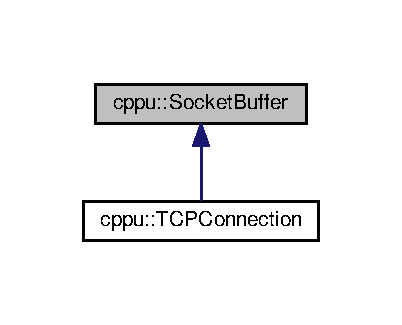
\includegraphics[width=193pt]{classcppu_1_1SocketBuffer__inherit__graph}
\end{center}
\end{figure}


Collaboration diagram for cppu\+:\+:Socket\+Buffer\+:
\nopagebreak
\begin{figure}[H]
\begin{center}
\leavevmode
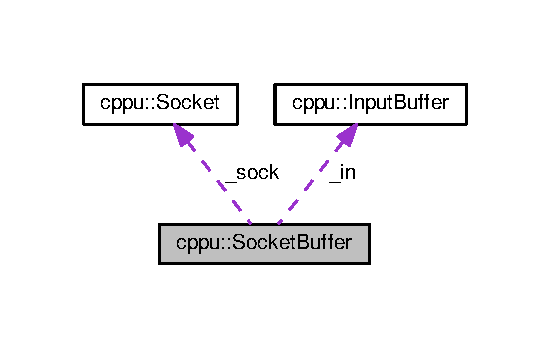
\includegraphics[width=264pt]{classcppu_1_1SocketBuffer__coll__graph}
\end{center}
\end{figure}
\subsection*{Public Member Functions}
\begin{DoxyCompactItemize}
\item 
\hypertarget{classcppu_1_1SocketBuffer_a1d6a8ae90bfcb69e6b3d2b9f97e3dc40}{\hyperlink{classcppu_1_1SocketBuffer_a1d6a8ae90bfcb69e6b3d2b9f97e3dc40}{Socket\+Buffer} (\hyperlink{classcppu_1_1Socket}{Socket} $\ast$\hyperlink{classcppu_1_1SocketBuffer_aab887b32ee999bfdd01c9a491c04bd61}{socket}, size\+\_\+t input\+Buffer\+Size=8192, size\+\_\+t ouput\+Buffer\+Size=8192)}\label{classcppu_1_1SocketBuffer_a1d6a8ae90bfcb69e6b3d2b9f97e3dc40}

\begin{DoxyCompactList}\small\item\em constructor. {\itshape socket} must be a connected T\+C\+P/\+I\+P \hyperlink{classcppu_1_1Socket}{Socket} (i.\+e. of S\+O\+C\+K\+\_\+\+S\+T\+R\+E\+A\+M type) that must {\itshape not} be deleted while the \hyperlink{classcppu_1_1SocketBuffer}{Socket\+Buffer} is used. {\itshape input\+Buffer\+Size} and {\itshape ouput\+Buffer\+Size} are the sizes of the buffers that used internally for exchanging the data. \end{DoxyCompactList}\item 
\hypertarget{classcppu_1_1SocketBuffer_ae8e387747f17f4ff3bfe036ccf11e89b}{{\bfseries Socket\+Buffer} (\hyperlink{classcppu_1_1Socket}{Socket} \&\hyperlink{classcppu_1_1SocketBuffer_aab887b32ee999bfdd01c9a491c04bd61}{socket}, size\+\_\+t input\+Buffer\+Size=8192, size\+\_\+t ouput\+Buffer\+Size=8192)}\label{classcppu_1_1SocketBuffer_ae8e387747f17f4ff3bfe036ccf11e89b}

\item 
\hypertarget{classcppu_1_1SocketBuffer_aab887b32ee999bfdd01c9a491c04bd61}{\hyperlink{classcppu_1_1Socket}{Socket} $\ast$ \hyperlink{classcppu_1_1SocketBuffer_aab887b32ee999bfdd01c9a491c04bd61}{socket} ()}\label{classcppu_1_1SocketBuffer_aab887b32ee999bfdd01c9a491c04bd61}

\begin{DoxyCompactList}\small\item\em returns the associated socket. \end{DoxyCompactList}\item 
\hypertarget{classcppu_1_1SocketBuffer_a77dfe31ad3d5660322d788daf213534e}{int \hyperlink{classcppu_1_1SocketBuffer_a77dfe31ad3d5660322d788daf213534e}{input\+Separator} () const }\label{classcppu_1_1SocketBuffer_a77dfe31ad3d5660322d788daf213534e}

\begin{DoxyCompactList}\small\item\em returns the input separator. \end{DoxyCompactList}\item 
\hypertarget{classcppu_1_1SocketBuffer_a737c72f4ce5ff73a2e7339430b6d1614}{int \hyperlink{classcppu_1_1SocketBuffer_a737c72f4ce5ff73a2e7339430b6d1614}{output\+Separator} () const }\label{classcppu_1_1SocketBuffer_a737c72f4ce5ff73a2e7339430b6d1614}

\begin{DoxyCompactList}\small\item\em returns the output separator. \end{DoxyCompactList}\item 
virtual void \hyperlink{classcppu_1_1SocketBuffer_acadf4540c1e3eba67b014753b84b482c}{set\+Input\+Separator} (int separ)
\begin{DoxyCompactList}\small\item\em changes the input separator. This function specifies the character(s) used by \hyperlink{classcppu_1_1SocketBuffer_a222769d3776b9cbd3a727ee1f0e60358}{read\+Line()} to separate successive lines\+: \end{DoxyCompactList}\item 
virtual void \hyperlink{classcppu_1_1SocketBuffer_a0e5e6a9ce3bda28b65c559c8b3c91b0f}{set\+Output\+Separator} (int separ)
\begin{DoxyCompactList}\small\item\em changes the output separator. This function specifies the character(s) used by \hyperlink{classcppu_1_1SocketBuffer_a92ae0351aaee8719d34e8c4618495d59}{write\+Line()} to separate successive lines\+: \end{DoxyCompactList}\item 
virtual ssize\+\_\+t \hyperlink{classcppu_1_1SocketBuffer_a222769d3776b9cbd3a727ee1f0e60358}{read\+Line} (std\+::string \&str)
\begin{DoxyCompactList}\small\item\em Reads a line of text from a connected socket. \hyperlink{classcppu_1_1SocketBuffer_a222769d3776b9cbd3a727ee1f0e60358}{read\+Line()} receives one line of text sent by \hyperlink{classcppu_1_1SocketBuffer_a92ae0351aaee8719d34e8c4618495d59}{write\+Line()} on the other side. The text is stored in {\itshape str}. This method blocks until the complete text line is received. \end{DoxyCompactList}\item 
virtual ssize\+\_\+t \hyperlink{classcppu_1_1SocketBuffer_a92ae0351aaee8719d34e8c4618495d59}{write\+Line} (const std\+::string \&str)
\begin{DoxyCompactList}\small\item\em Sends a line of text to a connected socket. \hyperlink{classcppu_1_1SocketBuffer_a92ae0351aaee8719d34e8c4618495d59}{write\+Line()} sends one line of text that will be received by a single call to \hyperlink{classcppu_1_1SocketBuffer_a222769d3776b9cbd3a727ee1f0e60358}{read\+Line()} on the other side (see note below). \end{DoxyCompactList}\item 
\hypertarget{classcppu_1_1SocketBuffer_a27de273ae2defbf3a5cc308310b9835e}{virtual ssize\+\_\+t {\bfseries read} (char $\ast$buffer, size\+\_\+t len)}\label{classcppu_1_1SocketBuffer_a27de273ae2defbf3a5cc308310b9835e}

\item 
\hypertarget{classcppu_1_1SocketBuffer_ab4ed032f329be2f6ecd0cba5fcd0518d}{virtual ssize\+\_\+t {\bfseries write} (const char $\ast$str, size\+\_\+t len)}\label{classcppu_1_1SocketBuffer_ab4ed032f329be2f6ecd0cba5fcd0518d}

\end{DoxyCompactItemize}
\subsection*{Protected Member Functions}
\begin{DoxyCompactItemize}
\item 
\hypertarget{classcppu_1_1SocketBuffer_ae634cbe12f6688a8d64c4579299e9802}{virtual bool {\bfseries retrieve\+Line} (std\+::string \&str, ssize\+\_\+t received)}\label{classcppu_1_1SocketBuffer_ae634cbe12f6688a8d64c4579299e9802}

\end{DoxyCompactItemize}
\subsection*{Protected Attributes}
\begin{DoxyCompactItemize}
\item 
\hypertarget{classcppu_1_1SocketBuffer_af52d0e7a5fb70ad371693c2e7f9f056b}{size\+\_\+t {\bfseries \+\_\+in\+Size}}\label{classcppu_1_1SocketBuffer_af52d0e7a5fb70ad371693c2e7f9f056b}

\item 
\hypertarget{classcppu_1_1SocketBuffer_afa2daeed2c8538030353382f48269896}{size\+\_\+t {\bfseries \+\_\+out\+Size}}\label{classcppu_1_1SocketBuffer_afa2daeed2c8538030353382f48269896}

\item 
\hypertarget{classcppu_1_1SocketBuffer_a5bf8f3a5ef56fc6f15ade71fe55b049d}{int {\bfseries \+\_\+in\+Sep}}\label{classcppu_1_1SocketBuffer_a5bf8f3a5ef56fc6f15ade71fe55b049d}

\item 
\hypertarget{classcppu_1_1SocketBuffer_a59b35cfa717476d18cc2e40c73073354}{int {\bfseries \+\_\+out\+Sep}}\label{classcppu_1_1SocketBuffer_a59b35cfa717476d18cc2e40c73073354}

\item 
\hypertarget{classcppu_1_1SocketBuffer_af60722acd94826d780bbb2477667d538}{\hyperlink{classcppu_1_1Socket}{Socket} $\ast$ {\bfseries \+\_\+sock}}\label{classcppu_1_1SocketBuffer_af60722acd94826d780bbb2477667d538}

\item 
\hypertarget{classcppu_1_1SocketBuffer_adb5986d6297496a1f92a30b1b3923072}{struct \hyperlink{structcppu_1_1InputBuffer}{Input\+Buffer} $\ast$ {\bfseries \+\_\+in}}\label{classcppu_1_1SocketBuffer_adb5986d6297496a1f92a30b1b3923072}

\end{DoxyCompactItemize}


\subsection{Detailed Description}
Preserves record boundaries when exchanging data between connected T\+C\+P/\+I\+P sockets. This class ensures that one call to \hyperlink{classcppu_1_1SocketBuffer_a92ae0351aaee8719d34e8c4618495d59}{write\+Line()} corresponds to one and exactly one call to \hyperlink{classcppu_1_1SocketBuffer_a222769d3776b9cbd3a727ee1f0e60358}{read\+Line()} on the other side. This differs from the behavior of \hyperlink{classcppu_1_1Socket_aeac77f859159715e2d63a5a0dc118788}{Socket\+::send()} and \hyperlink{classcppu_1_1Socket_a37c382af52cc02f92c0e19a0c6e0e04f}{Socket\+::receive()} because T\+C\+P/\+I\+P connected sockets do not preserve record boundaries. \hyperlink{classcppu_1_1SocketBuffer_a92ae0351aaee8719d34e8c4618495d59}{write\+Line()} and \hyperlink{classcppu_1_1SocketBuffer_a222769d3776b9cbd3a727ee1f0e60358}{read\+Line()} solve this problem by automatically adding and searching for a separator between successive lines. 

\begin{DoxySeeAlso}{See also}
\hyperlink{classcppu_1_1SocketBuffer_acadf4540c1e3eba67b014753b84b482c}{set\+Input\+Separator()} and \hyperlink{classcppu_1_1SocketBuffer_a0e5e6a9ce3bda28b65c559c8b3c91b0f}{set\+Output\+Separator()}. 
\end{DoxySeeAlso}


\subsection{Member Function Documentation}
\hypertarget{classcppu_1_1SocketBuffer_a222769d3776b9cbd3a727ee1f0e60358}{\index{cppu\+::\+Socket\+Buffer@{cppu\+::\+Socket\+Buffer}!read\+Line@{read\+Line}}
\index{read\+Line@{read\+Line}!cppu\+::\+Socket\+Buffer@{cppu\+::\+Socket\+Buffer}}
\subsubsection[{read\+Line}]{\setlength{\rightskip}{0pt plus 5cm}ssize\+\_\+t cppu\+::\+Socket\+Buffer\+::read\+Line (
\begin{DoxyParamCaption}
\item[{std\+::string \&}]{str}
\end{DoxyParamCaption}
)\hspace{0.3cm}{\ttfamily [virtual]}}}\label{classcppu_1_1SocketBuffer_a222769d3776b9cbd3a727ee1f0e60358}


Reads a line of text from a connected socket. \hyperlink{classcppu_1_1SocketBuffer_a222769d3776b9cbd3a727ee1f0e60358}{read\+Line()} receives one line of text sent by \hyperlink{classcppu_1_1SocketBuffer_a92ae0351aaee8719d34e8c4618495d59}{write\+Line()} on the other side. The text is stored in {\itshape str}. This method blocks until the complete text line is received. 

\hyperlink{classcppu_1_1SocketBuffer_a222769d3776b9cbd3a727ee1f0e60358}{read\+Line()} relies on a separator (by default, ~\newline
, ~\newline
 or ~\newline
, \begin{DoxySeeAlso}{See also}
\hyperlink{classcppu_1_1SocketBuffer_acadf4540c1e3eba67b014753b84b482c}{set\+Input\+Separator()}. This separator is automatically removed (it is not stored in {\itshape str}).
\end{DoxySeeAlso}
\begin{DoxyReturn}{Returns}
the number of bytes that were received or\+:
\begin{DoxyItemize}
\item 0\+: shutdown\+Output() was called on the other side
\item Socket\+::\+Failed (-\/1)\+: a connection error occured
\item Socket\+::\+Invalid\+Socket (-\/2)\+: the socket is invalid. The separator is counted in the value returned by \hyperlink{classcppu_1_1SocketBuffer_a222769d3776b9cbd3a727ee1f0e60358}{read\+Line()}. 
\end{DoxyItemize}
\end{DoxyReturn}
\hypertarget{classcppu_1_1SocketBuffer_acadf4540c1e3eba67b014753b84b482c}{\index{cppu\+::\+Socket\+Buffer@{cppu\+::\+Socket\+Buffer}!set\+Input\+Separator@{set\+Input\+Separator}}
\index{set\+Input\+Separator@{set\+Input\+Separator}!cppu\+::\+Socket\+Buffer@{cppu\+::\+Socket\+Buffer}}
\subsubsection[{set\+Input\+Separator}]{\setlength{\rightskip}{0pt plus 5cm}void cppu\+::\+Socket\+Buffer\+::set\+Input\+Separator (
\begin{DoxyParamCaption}
\item[{int}]{separ}
\end{DoxyParamCaption}
)\hspace{0.3cm}{\ttfamily [virtual]}}}\label{classcppu_1_1SocketBuffer_acadf4540c1e3eba67b014753b84b482c}


changes the input separator. This function specifies the character(s) used by \hyperlink{classcppu_1_1SocketBuffer_a222769d3776b9cbd3a727ee1f0e60358}{read\+Line()} to separate successive lines\+: 


\begin{DoxyItemize}
\item if {\itshape separ} $>$= 0, \hyperlink{classcppu_1_1SocketBuffer_a222769d3776b9cbd3a727ee1f0e60358}{read\+Line()} searches for {\itshape separ} to separate lines,
\item if {\itshape separ} $<$ 0, \hyperlink{classcppu_1_1SocketBuffer_a222769d3776b9cbd3a727ee1f0e60358}{read\+Line()} searches for ~\newline
,  or ~\newline
. By default, \hyperlink{classcppu_1_1SocketBuffer_a222769d3776b9cbd3a727ee1f0e60358}{read\+Line()} for ~\newline
,  or ~\newline
. \begin{DoxyNote}{Note}
If the input separator is changed, the output separator must be changed accordingly on the other side of the socket. 
\end{DoxyNote}
\begin{DoxySeeAlso}{See also}
\hyperlink{classcppu_1_1SocketBuffer_a0e5e6a9ce3bda28b65c559c8b3c91b0f}{set\+Output\+Separator()}. 
\end{DoxySeeAlso}

\end{DoxyItemize}\hypertarget{classcppu_1_1SocketBuffer_a0e5e6a9ce3bda28b65c559c8b3c91b0f}{\index{cppu\+::\+Socket\+Buffer@{cppu\+::\+Socket\+Buffer}!set\+Output\+Separator@{set\+Output\+Separator}}
\index{set\+Output\+Separator@{set\+Output\+Separator}!cppu\+::\+Socket\+Buffer@{cppu\+::\+Socket\+Buffer}}
\subsubsection[{set\+Output\+Separator}]{\setlength{\rightskip}{0pt plus 5cm}void cppu\+::\+Socket\+Buffer\+::set\+Output\+Separator (
\begin{DoxyParamCaption}
\item[{int}]{separ}
\end{DoxyParamCaption}
)\hspace{0.3cm}{\ttfamily [virtual]}}}\label{classcppu_1_1SocketBuffer_a0e5e6a9ce3bda28b65c559c8b3c91b0f}


changes the output separator. This function specifies the character(s) used by \hyperlink{classcppu_1_1SocketBuffer_a92ae0351aaee8719d34e8c4618495d59}{write\+Line()} to separate successive lines\+: 


\begin{DoxyItemize}
\item if {\itshape separ} $>$= 0, \hyperlink{classcppu_1_1SocketBuffer_a92ae0351aaee8719d34e8c4618495d59}{write\+Line()} inserts {\itshape separ} between successive lines,
\item if {\itshape separ} $<$ 0, \hyperlink{classcppu_1_1SocketBuffer_a92ae0351aaee8719d34e8c4618495d59}{write\+Line()} inserts ~\newline
 between successive lines. By default, \hyperlink{classcppu_1_1SocketBuffer_a92ae0351aaee8719d34e8c4618495d59}{write\+Line()} inserts ~\newline
. \begin{DoxyNote}{Note}
If the output separator is changed, the input separator must be changed accordingly on the other side of the socket. 
\end{DoxyNote}
\begin{DoxySeeAlso}{See also}
\hyperlink{classcppu_1_1SocketBuffer_acadf4540c1e3eba67b014753b84b482c}{set\+Input\+Separator()}. 
\end{DoxySeeAlso}

\end{DoxyItemize}\hypertarget{classcppu_1_1SocketBuffer_a92ae0351aaee8719d34e8c4618495d59}{\index{cppu\+::\+Socket\+Buffer@{cppu\+::\+Socket\+Buffer}!write\+Line@{write\+Line}}
\index{write\+Line@{write\+Line}!cppu\+::\+Socket\+Buffer@{cppu\+::\+Socket\+Buffer}}
\subsubsection[{write\+Line}]{\setlength{\rightskip}{0pt plus 5cm}ssize\+\_\+t cppu\+::\+Socket\+Buffer\+::write\+Line (
\begin{DoxyParamCaption}
\item[{const std\+::string \&}]{str}
\end{DoxyParamCaption}
)\hspace{0.3cm}{\ttfamily [virtual]}}}\label{classcppu_1_1SocketBuffer_a92ae0351aaee8719d34e8c4618495d59}


Sends a line of text to a connected socket. \hyperlink{classcppu_1_1SocketBuffer_a92ae0351aaee8719d34e8c4618495d59}{write\+Line()} sends one line of text that will be received by a single call to \hyperlink{classcppu_1_1SocketBuffer_a222769d3776b9cbd3a727ee1f0e60358}{read\+Line()} on the other side (see note below). 

\hyperlink{classcppu_1_1SocketBuffer_a92ae0351aaee8719d34e8c4618495d59}{write\+Line()} relies on a separator (~\newline
 by default, \begin{DoxySeeAlso}{See also}
\hyperlink{classcppu_1_1SocketBuffer_a0e5e6a9ce3bda28b65c559c8b3c91b0f}{set\+Output\+Separator()}) that is automatically inserted between successive lines ().
\end{DoxySeeAlso}
\begin{DoxyReturn}{Returns}
the number of bytes that were sent or\+:
\begin{DoxyItemize}
\item 0\+: shutdown\+Input() was called on the other side
\item Socket\+::\+Failed (-\/1)\+: a connection error occured
\item Socket\+::\+Invalid\+Socket (-\/2)\+: the socket is invalid. The separator is counted in the value returned by \hyperlink{classcppu_1_1SocketBuffer_a92ae0351aaee8719d34e8c4618495d59}{write\+Line()}.
\end{DoxyItemize}
\end{DoxyReturn}
\begin{DoxyNote}{Note}
if {\itshape str} constains occurences of the separator, \hyperlink{classcppu_1_1SocketBuffer_a222769d3776b9cbd3a727ee1f0e60358}{read\+Line()} will be called several times on the other side. 
\end{DoxyNote}


The documentation for this class was generated from the following files\+:\begin{DoxyCompactItemize}
\item 
cppsocket.\+h\item 
cppsocket.\+cpp\end{DoxyCompactItemize}

\hypertarget{classcppu_1_1TCPConnection}{\section{cppu\+:\+:T\+C\+P\+Connection Class Reference}
\label{classcppu_1_1TCPConnection}\index{cppu\+::\+T\+C\+P\+Connection@{cppu\+::\+T\+C\+P\+Connection}}
}


Connection with a given client. Each \hyperlink{classcppu_1_1TCPConnection}{T\+C\+P\+Connection} uses a different thread.  




{\ttfamily \#include $<$tcpserver.\+h$>$}



Inheritance diagram for cppu\+:\+:T\+C\+P\+Connection\+:
\nopagebreak
\begin{figure}[H]
\begin{center}
\leavevmode
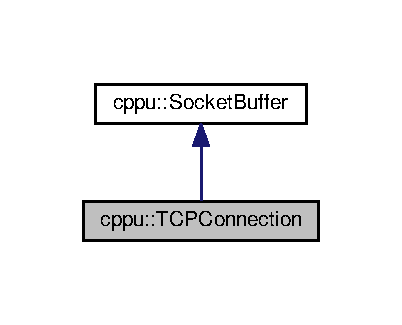
\includegraphics[width=193pt]{classcppu_1_1TCPConnection__inherit__graph}
\end{center}
\end{figure}


Collaboration diagram for cppu\+:\+:T\+C\+P\+Connection\+:
\nopagebreak
\begin{figure}[H]
\begin{center}
\leavevmode
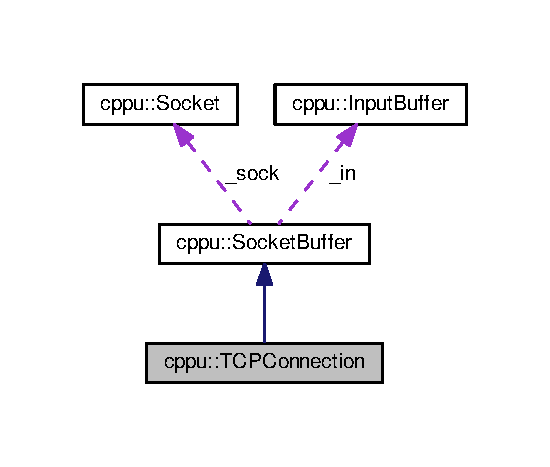
\includegraphics[width=264pt]{classcppu_1_1TCPConnection__coll__graph}
\end{center}
\end{figure}
\subsection*{Public Member Functions}
\begin{DoxyCompactItemize}
\item 
\hypertarget{classcppu_1_1TCPConnection_a4186946c7c22e3c2cebe3a97aa78f5f7}{\hyperlink{classcppu_1_1TCPServer}{T\+C\+P\+Server} \& {\bfseries server} ()}\label{classcppu_1_1TCPConnection_a4186946c7c22e3c2cebe3a97aa78f5f7}

\item 
\hypertarget{classcppu_1_1TCPConnection_a4663875b80fced790502880c72e6e672}{pthread\+\_\+t {\bfseries thread} ()}\label{classcppu_1_1TCPConnection_a4663875b80fced790502880c72e6e672}

\end{DoxyCompactItemize}
\subsection*{Friends}
\begin{DoxyCompactItemize}
\item 
\hypertarget{classcppu_1_1TCPConnection_ae4cfdb1814d91a8d28dadb49adda68f0}{class {\bfseries T\+C\+P\+Server}}\label{classcppu_1_1TCPConnection_ae4cfdb1814d91a8d28dadb49adda68f0}

\end{DoxyCompactItemize}
\subsection*{Additional Inherited Members}


\subsection{Detailed Description}
Connection with a given client. Each \hyperlink{classcppu_1_1TCPConnection}{T\+C\+P\+Connection} uses a different thread. 

The documentation for this class was generated from the following files\+:\begin{DoxyCompactItemize}
\item 
tcpserver.\+h\item 
tcpserver.\+cpp\end{DoxyCompactItemize}

\hypertarget{classcppu_1_1TCPLock}{\section{cppu\+:\+:T\+C\+P\+Lock Class Reference}
\label{classcppu_1_1TCPLock}\index{cppu\+::\+T\+C\+P\+Lock@{cppu\+::\+T\+C\+P\+Lock}}
}


Locks the server in read mode or in write mode. Must be created {\itshape in the stack} by the callback method.  




{\ttfamily \#include $<$tcpserver.\+h$>$}

\subsection*{Public Member Functions}
\begin{DoxyCompactItemize}
\item 
\hyperlink{classcppu_1_1TCPLock_ad9ff8205f334918a69746ef90f731877}{T\+C\+P\+Lock} (\hyperlink{classcppu_1_1TCPConnection}{T\+C\+P\+Connection} \&cnx, bool write\+Mode=false)
\begin{DoxyCompactList}\small\item\em locks the server in {\itshape write} or {\itshape read} mode. In order to avoid concurrency problems between threads, the callback method ( \end{DoxyCompactList}\end{DoxyCompactItemize}


\subsection{Detailed Description}
Locks the server in read mode or in write mode. Must be created {\itshape in the stack} by the callback method. 

\subsection{Constructor \& Destructor Documentation}
\hypertarget{classcppu_1_1TCPLock_ad9ff8205f334918a69746ef90f731877}{\index{cppu\+::\+T\+C\+P\+Lock@{cppu\+::\+T\+C\+P\+Lock}!T\+C\+P\+Lock@{T\+C\+P\+Lock}}
\index{T\+C\+P\+Lock@{T\+C\+P\+Lock}!cppu\+::\+T\+C\+P\+Lock@{cppu\+::\+T\+C\+P\+Lock}}
\subsubsection[{T\+C\+P\+Lock}]{\setlength{\rightskip}{0pt plus 5cm}cppu\+::\+T\+C\+P\+Lock\+::\+T\+C\+P\+Lock (
\begin{DoxyParamCaption}
\item[{{\bf T\+C\+P\+Connection} \&}]{cnx, }
\item[{bool}]{write\+Mode = {\ttfamily false}}
\end{DoxyParamCaption}
)}}\label{classcppu_1_1TCPLock_ad9ff8205f334918a69746ef90f731877}


locks the server in {\itshape write} or {\itshape read} mode. In order to avoid concurrency problems between threads, the callback method ( 

\begin{DoxySeeAlso}{See also}
set\+Callback()) can create a \hyperlink{classcppu_1_1TCPLock}{T\+C\+P\+Lock} object {\itshape in the stack} before performing a computation.
\end{DoxySeeAlso}
{\itshape write\+Mode} must be true if the callback changes data and false (the default) otherwise. A write\+Mode lock blocks all other locks (and the corresponding threads) until the callback method returns. 

The documentation for this class was generated from the following files\+:\begin{DoxyCompactItemize}
\item 
tcpserver.\+h\item 
tcpserver.\+cpp\end{DoxyCompactItemize}

\hypertarget{classcppu_1_1TCPServer}{\section{cppu\+:\+:T\+C\+P\+Server Class Reference}
\label{classcppu_1_1TCPServer}\index{cppu\+::\+T\+C\+P\+Server@{cppu\+::\+T\+C\+P\+Server}}
}


T\+C\+P/\+I\+P I\+Pv4 server. The server supports T\+C\+P/\+I\+P A\+F\+\_\+\+I\+N\+E\+T connections (following the I\+Pv4 Internet protocol) with multiple clients. One thread is used per client.  




{\ttfamily \#include $<$tcpserver.\+h$>$}



Collaboration diagram for cppu\+:\+:T\+C\+P\+Server\+:
\nopagebreak
\begin{figure}[H]
\begin{center}
\leavevmode
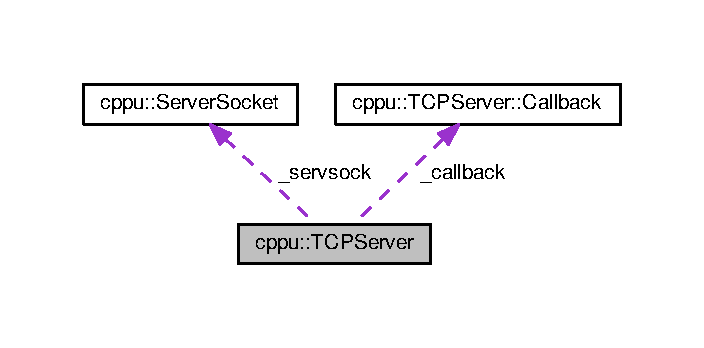
\includegraphics[width=338pt]{classcppu_1_1TCPServer__coll__graph}
\end{center}
\end{figure}
\subsection*{Classes}
\begin{DoxyCompactItemize}
\item 
struct \hyperlink{structcppu_1_1TCPServer_1_1Callback}{Callback}
\begin{DoxyCompactList}\small\item\em \hyperlink{structcppu_1_1TCPServer_1_1Callback}{Callback} interface. \end{DoxyCompactList}\item 
struct \hyperlink{structcppu_1_1TCPServer_1_1CallbackMethod}{Callback\+Method}
\end{DoxyCompactItemize}
\subsection*{Public Member Functions}
\begin{DoxyCompactItemize}
\item 
\hypertarget{classcppu_1_1TCPServer_a48074f8409f580f6cf7b0be80200f9f3}{\hyperlink{classcppu_1_1TCPServer_a48074f8409f580f6cf7b0be80200f9f3}{T\+C\+P\+Server} ()}\label{classcppu_1_1TCPServer_a48074f8409f580f6cf7b0be80200f9f3}

\begin{DoxyCompactList}\small\item\em constructor\+: initializes the \hyperlink{classcppu_1_1TCPServer}{T\+C\+P\+Server}. \end{DoxyCompactList}\item 
\hypertarget{classcppu_1_1TCPServer_ababd20111e0cf4e14396433e56ca086e}{virtual \hyperlink{classcppu_1_1TCPServer_ababd20111e0cf4e14396433e56ca086e}{$\sim$\+T\+C\+P\+Server} ()}\label{classcppu_1_1TCPServer_ababd20111e0cf4e14396433e56ca086e}

\begin{DoxyCompactList}\small\item\em destructor\+: cleans up the \hyperlink{classcppu_1_1TCPServer}{T\+C\+P\+Server}. \end{DoxyCompactList}\item 
virtual int \hyperlink{classcppu_1_1TCPServer_a98e00d62745812b17bdee9f07f2070c4}{run} (int port)
\begin{DoxyCompactList}\small\item\em starts the \hyperlink{classcppu_1_1TCPServer}{T\+C\+P\+Server}. \hyperlink{classcppu_1_1TCPServer_a98e00d62745812b17bdee9f07f2070c4}{run()} binds an internal \hyperlink{classcppu_1_1ServerSocket}{Server\+Socket} to {\itshape port} then starts an infinite loop that processes connection requests from clients. \end{DoxyCompactList}\item 
{\footnotesize template$<$class T $>$ }\\void \hyperlink{classcppu_1_1TCPServer_a7d4fdb93439015934004755fde72945b}{set\+Callback} (T \&object, bool(T\+::$\ast$method)(\hyperlink{classcppu_1_1TCPConnection}{T\+C\+P\+Connection} \&cnx, const std\+::string \&request, std\+::string \&response))
\begin{DoxyCompactList}\small\item\em changes the callback method of the \hyperlink{classcppu_1_1TCPServer}{T\+C\+P\+Server}. This callback is called each time the \hyperlink{classcppu_1_1TCPServer}{T\+C\+P\+Server} receives a request from a client. It can be any method of {\itshape object} with the following parameters\+: \end{DoxyCompactList}\item 
void \hyperlink{classcppu_1_1TCPServer_a94d3d97b03d5e3e48609e405d8dd7897}{set\+Callback} (\hyperlink{structcppu_1_1TCPServer_1_1Callback}{Callback} \&callback)
\begin{DoxyCompactList}\small\item\em changes the callback object of the \hyperlink{classcppu_1_1TCPServer}{T\+C\+P\+Server}. \end{DoxyCompactList}\item 
\hypertarget{classcppu_1_1TCPServer_a6428b63a4440045050dba4f33bb454bf}{\hyperlink{classcppu_1_1ServerSocket}{Server\+Socket} \& \hyperlink{classcppu_1_1TCPServer_a6428b63a4440045050dba4f33bb454bf}{server\+Socket} ()}\label{classcppu_1_1TCPServer_a6428b63a4440045050dba4f33bb454bf}

\begin{DoxyCompactList}\small\item\em returns the internal \hyperlink{classcppu_1_1ServerSocket}{Server\+Socket}. \end{DoxyCompactList}\item 
\hypertarget{classcppu_1_1TCPServer_afc47ca4476d9c75d5ea88f73e2acd6d5}{virtual void \hyperlink{classcppu_1_1TCPServer_afc47ca4476d9c75d5ea88f73e2acd6d5}{error} (const std\+::string \&msg, const \hyperlink{classcppu_1_1TCPConnection}{T\+C\+P\+Connection} $\ast$=nullptr)}\label{classcppu_1_1TCPServer_afc47ca4476d9c75d5ea88f73e2acd6d5}

\begin{DoxyCompactList}\small\item\em prints warning and error messages on the terminal. \end{DoxyCompactList}\end{DoxyCompactItemize}
\subsection*{Protected Member Functions}
\begin{DoxyCompactItemize}
\item 
\hypertarget{classcppu_1_1TCPServer_abe314b95a31c88b479c81ec9bf123c65}{virtual \hyperlink{classcppu_1_1TCPConnection}{T\+C\+P\+Connection} $\ast$ \hyperlink{classcppu_1_1TCPServer_abe314b95a31c88b479c81ec9bf123c65}{create\+Cnx} (\hyperlink{classcppu_1_1Socket}{Socket} $\ast$)}\label{classcppu_1_1TCPServer_abe314b95a31c88b479c81ec9bf123c65}

\begin{DoxyCompactList}\small\item\em creates a new connection that starts a new thread for listening this socket. \end{DoxyCompactList}\end{DoxyCompactItemize}
\subsection*{Protected Attributes}
\begin{DoxyCompactItemize}
\item 
\hypertarget{classcppu_1_1TCPServer_a8e4422abf23dc5bd195d05a3e9eee167}{\hyperlink{classcppu_1_1ServerSocket}{Server\+Socket} {\bfseries \+\_\+servsock}}\label{classcppu_1_1TCPServer_a8e4422abf23dc5bd195d05a3e9eee167}

\item 
\hypertarget{classcppu_1_1TCPServer_abe36d427d7b047cdd342e282611c841e}{std\+::shared\+\_\+ptr$<$ \hyperlink{structcppu_1_1TCPServer_1_1Callback}{Callback} $>$ {\bfseries \+\_\+callback\+Ptr}}\label{classcppu_1_1TCPServer_abe36d427d7b047cdd342e282611c841e}

\item 
\hypertarget{classcppu_1_1TCPServer_a68940bd70ac6941ca49d1e51b631f5e9}{\hyperlink{structcppu_1_1TCPServer_1_1Callback}{Callback} $\ast$ {\bfseries \+\_\+callback}}\label{classcppu_1_1TCPServer_a68940bd70ac6941ca49d1e51b631f5e9}

\item 
\hypertarget{classcppu_1_1TCPServer_aea2dbb4b5762044217096e52cd559b97}{pthread\+\_\+rwlock\+\_\+t {\bfseries \+\_\+threadlock}}\label{classcppu_1_1TCPServer_aea2dbb4b5762044217096e52cd559b97}

\end{DoxyCompactItemize}
\subsection*{Friends}
\begin{DoxyCompactItemize}
\item 
\hypertarget{classcppu_1_1TCPServer_a94abdeb80587f39a869fde6f24522a78}{class {\bfseries T\+C\+P\+Lock}}\label{classcppu_1_1TCPServer_a94abdeb80587f39a869fde6f24522a78}

\item 
\hypertarget{classcppu_1_1TCPServer_a9d1c27bdfcdd48c5f07a5d0dce43b346}{class {\bfseries T\+C\+P\+Connection}}\label{classcppu_1_1TCPServer_a9d1c27bdfcdd48c5f07a5d0dce43b346}

\end{DoxyCompactItemize}


\subsection{Detailed Description}
T\+C\+P/\+I\+P I\+Pv4 server. The server supports T\+C\+P/\+I\+P A\+F\+\_\+\+I\+N\+E\+T connections (following the I\+Pv4 Internet protocol) with multiple clients. One thread is used per client. 

Call \hyperlink{classcppu_1_1TCPServer_a7d4fdb93439015934004755fde72945b}{set\+Callback()} to specify the callback method that will be invoked each time a request is sent by a client then \hyperlink{classcppu_1_1TCPServer_a98e00d62745812b17bdee9f07f2070c4}{run()} to start the server.

Requests can be processed concurrently thanks to threads. To avoid concurrency problems the callback can perform a read or write lock (\begin{DoxySeeAlso}{See also}
\hyperlink{classcppu_1_1TCPLock}{T\+C\+P\+Lock}). 
\end{DoxySeeAlso}


\subsection{Member Function Documentation}
\hypertarget{classcppu_1_1TCPServer_a98e00d62745812b17bdee9f07f2070c4}{\index{cppu\+::\+T\+C\+P\+Server@{cppu\+::\+T\+C\+P\+Server}!run@{run}}
\index{run@{run}!cppu\+::\+T\+C\+P\+Server@{cppu\+::\+T\+C\+P\+Server}}
\subsubsection[{run}]{\setlength{\rightskip}{0pt plus 5cm}int cppu\+::\+T\+C\+P\+Server\+::run (
\begin{DoxyParamCaption}
\item[{int}]{port}
\end{DoxyParamCaption}
)\hspace{0.3cm}{\ttfamily [virtual]}}}\label{classcppu_1_1TCPServer_a98e00d62745812b17bdee9f07f2070c4}


starts the \hyperlink{classcppu_1_1TCPServer}{T\+C\+P\+Server}. \hyperlink{classcppu_1_1TCPServer_a98e00d62745812b17bdee9f07f2070c4}{run()} binds an internal \hyperlink{classcppu_1_1ServerSocket}{Server\+Socket} to {\itshape port} then starts an infinite loop that processes connection requests from clients. 

For each successful connection request, a \hyperlink{classcppu_1_1TCPConnection}{T\+C\+P\+Connection} object is created. This object starts a thread that processes incoming requests from its client. A callback method (\begin{DoxySeeAlso}{See also}
\hyperlink{classcppu_1_1TCPServer_a7d4fdb93439015934004755fde72945b}{set\+Callback()}) is invoked for each request.
\end{DoxySeeAlso}
\begin{DoxyReturn}{Returns}
0 on normal termination or a negative value if the \hyperlink{classcppu_1_1ServerSocket}{Server\+Socket} could not be bound (value is then one of \hyperlink{classcppu_1_1Socket_a49ea5cb079bd7ae97ecf7eb30c9d9e5f}{Socket\+::\+Errors}). 
\end{DoxyReturn}
\hypertarget{classcppu_1_1TCPServer_a7d4fdb93439015934004755fde72945b}{\index{cppu\+::\+T\+C\+P\+Server@{cppu\+::\+T\+C\+P\+Server}!set\+Callback@{set\+Callback}}
\index{set\+Callback@{set\+Callback}!cppu\+::\+T\+C\+P\+Server@{cppu\+::\+T\+C\+P\+Server}}
\subsubsection[{set\+Callback}]{\setlength{\rightskip}{0pt plus 5cm}template$<$class T $>$ void cppu\+::\+T\+C\+P\+Server\+::set\+Callback (
\begin{DoxyParamCaption}
\item[{T \&}]{object, }
\item[{bool(T\+::$\ast$)({\bf T\+C\+P\+Connection} \&cnx, const std\+::string \&request, std\+::string \&response)}]{method}
\end{DoxyParamCaption}
)\hspace{0.3cm}{\ttfamily [inline]}}}\label{classcppu_1_1TCPServer_a7d4fdb93439015934004755fde72945b}


changes the callback method of the \hyperlink{classcppu_1_1TCPServer}{T\+C\+P\+Server}. This callback is called each time the \hyperlink{classcppu_1_1TCPServer}{T\+C\+P\+Server} receives a request from a client. It can be any method of {\itshape object} with the following parameters\+: 


\begin{DoxyItemize}
\item {\itshape cnx} is the connection with the client sending the request
\item {\itshape request} contains the data sent by the client
\item {\itshape response} will be sent to the client as a response The connection is closed if the callback returns false.
\end{DoxyItemize}

To avoid concurrency problems, the callback should perform a read or write lock (\begin{DoxySeeAlso}{See also}
\hyperlink{classcppu_1_1TCPLock}{T\+C\+P\+Lock}) before performing a computation. 
\end{DoxySeeAlso}
\hypertarget{classcppu_1_1TCPServer_a94d3d97b03d5e3e48609e405d8dd7897}{\index{cppu\+::\+T\+C\+P\+Server@{cppu\+::\+T\+C\+P\+Server}!set\+Callback@{set\+Callback}}
\index{set\+Callback@{set\+Callback}!cppu\+::\+T\+C\+P\+Server@{cppu\+::\+T\+C\+P\+Server}}
\subsubsection[{set\+Callback}]{\setlength{\rightskip}{0pt plus 5cm}void cppu\+::\+T\+C\+P\+Server\+::set\+Callback (
\begin{DoxyParamCaption}
\item[{{\bf Callback} \&}]{callback}
\end{DoxyParamCaption}
)\hspace{0.3cm}{\ttfamily [inline]}}}\label{classcppu_1_1TCPServer_a94d3d97b03d5e3e48609e405d8dd7897}


changes the callback object of the \hyperlink{classcppu_1_1TCPServer}{T\+C\+P\+Server}. 

\begin{DoxySeeAlso}{See also}
set\+Callback(object, method). 
\end{DoxySeeAlso}


The documentation for this class was generated from the following files\+:\begin{DoxyCompactItemize}
\item 
tcpserver.\+h\item 
tcpserver.\+cpp\end{DoxyCompactItemize}

\hypertarget{classVideo}{\section{Video Class Reference}
\label{classVideo}\index{Video@{Video}}
}


Inheritance diagram for Video\+:
\nopagebreak
\begin{figure}[H]
\begin{center}
\leavevmode
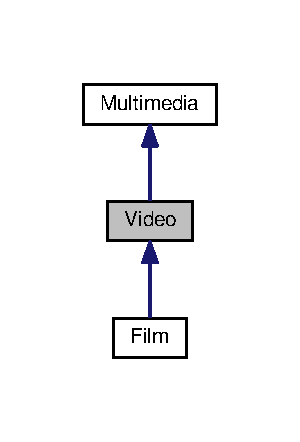
\includegraphics[width=144pt]{classVideo__inherit__graph}
\end{center}
\end{figure}


Collaboration diagram for Video\+:
\nopagebreak
\begin{figure}[H]
\begin{center}
\leavevmode
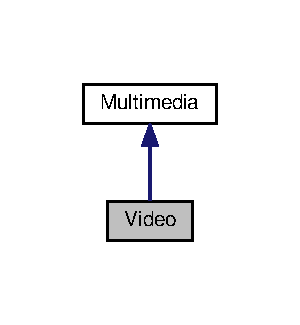
\includegraphics[width=144pt]{classVideo__coll__graph}
\end{center}
\end{figure}
\subsection*{Public Member Functions}
\begin{DoxyCompactItemize}
\item 
\hyperlink{classVideo_ae9c2fb1a73fb2882941f6d65100f5fc4}{Video} (string \+\_\+nom\+F=\char`\"{}\char`\"{}, string \+\_\+nom\+M=\char`\"{}\char`\"{}, int \+\_\+duree=0)
\begin{DoxyCompactList}\small\item\em \hyperlink{classVideo}{Video}. \end{DoxyCompactList}\item 
virtual int \hyperlink{classVideo_a481a3fe9717c76c2d012498c7a1b08ca}{get\+Duree} () const 
\begin{DoxyCompactList}\small\item\em get\+Duree \end{DoxyCompactList}\item 
virtual void \hyperlink{classVideo_a713899ce1fcf112a04ea18f917a60fa2}{set\+Duree} (int \+\_\+duree)
\begin{DoxyCompactList}\small\item\em set\+Duree \end{DoxyCompactList}\item 
virtual void \hyperlink{classVideo_a2f1902c8131fc232926e34487b54e0b9}{display} (ostream \&out, bool flag=false)
\begin{DoxyCompactList}\small\item\em display \end{DoxyCompactList}\item 
virtual void \hyperlink{classVideo_acb8fdb5186d3b35672b9218375cf4f0b}{play} () const 
\begin{DoxyCompactList}\small\item\em play \end{DoxyCompactList}\end{DoxyCompactItemize}
\subsection*{Additional Inherited Members}


\subsection{Constructor \& Destructor Documentation}
\hypertarget{classVideo_ae9c2fb1a73fb2882941f6d65100f5fc4}{\index{Video@{Video}!Video@{Video}}
\index{Video@{Video}!Video@{Video}}
\subsubsection[{Video}]{\setlength{\rightskip}{0pt plus 5cm}Video\+::\+Video (
\begin{DoxyParamCaption}
\item[{string}]{\+\_\+nom\+F = {\ttfamily \char`\"{}\char`\"{}}, }
\item[{string}]{\+\_\+nom\+M = {\ttfamily \char`\"{}\char`\"{}}, }
\item[{int}]{\+\_\+duree = {\ttfamily 0}}
\end{DoxyParamCaption}
)}}\label{classVideo_ae9c2fb1a73fb2882941f6d65100f5fc4}


\hyperlink{classVideo}{Video}. 


\begin{DoxyParams}{Parameters}
{\em } & return  initializer nom\+Fichier, nom\+Media, duree with parameter and inherit the constructer of multimedia \\
\hline
\end{DoxyParams}


\subsection{Member Function Documentation}
\hypertarget{classVideo_a2f1902c8131fc232926e34487b54e0b9}{\index{Video@{Video}!display@{display}}
\index{display@{display}!Video@{Video}}
\subsubsection[{display}]{\setlength{\rightskip}{0pt plus 5cm}void Video\+::display (
\begin{DoxyParamCaption}
\item[{ostream \&}]{out, }
\item[{bool}]{flag = {\ttfamily false}}
\end{DoxyParamCaption}
)\hspace{0.3cm}{\ttfamily [virtual]}}}\label{classVideo_a2f1902c8131fc232926e34487b54e0b9}


display 


\begin{DoxyParams}{Parameters}
{\em out,flag} & \\
\hline
\end{DoxyParams}
\begin{DoxyReturn}{Returns}
show the information of the video, flag is to judge if it is used for cout or server 
\end{DoxyReturn}


Reimplemented from \hyperlink{classMultimedia_a47176f027bfb92e5374cf34f4c70809a}{Multimedia}.



Reimplemented in \hyperlink{classFilm_a9f6a67ac8aa1e16501676c70e35d4eb4}{Film}.

\hypertarget{classVideo_a481a3fe9717c76c2d012498c7a1b08ca}{\index{Video@{Video}!get\+Duree@{get\+Duree}}
\index{get\+Duree@{get\+Duree}!Video@{Video}}
\subsubsection[{get\+Duree}]{\setlength{\rightskip}{0pt plus 5cm}int Video\+::get\+Duree (
\begin{DoxyParamCaption}
{}
\end{DoxyParamCaption}
) const\hspace{0.3cm}{\ttfamily [virtual]}}}\label{classVideo_a481a3fe9717c76c2d012498c7a1b08ca}


get\+Duree 


\begin{DoxyParams}{Parameters}
{\em } & return duree  get the value of duree \\
\hline
\end{DoxyParams}
\hypertarget{classVideo_acb8fdb5186d3b35672b9218375cf4f0b}{\index{Video@{Video}!play@{play}}
\index{play@{play}!Video@{Video}}
\subsubsection[{play}]{\setlength{\rightskip}{0pt plus 5cm}void Video\+::play (
\begin{DoxyParamCaption}
{}
\end{DoxyParamCaption}
) const\hspace{0.3cm}{\ttfamily [virtual]}}}\label{classVideo_acb8fdb5186d3b35672b9218375cf4f0b}


play 


\begin{DoxyParams}{Parameters}
{\em } & return  show the video \\
\hline
\end{DoxyParams}


Implements \hyperlink{classMultimedia_ad08d517e03460d941915682e8d0a13be}{Multimedia}.

\hypertarget{classVideo_a713899ce1fcf112a04ea18f917a60fa2}{\index{Video@{Video}!set\+Duree@{set\+Duree}}
\index{set\+Duree@{set\+Duree}!Video@{Video}}
\subsubsection[{set\+Duree}]{\setlength{\rightskip}{0pt plus 5cm}void Video\+::set\+Duree (
\begin{DoxyParamCaption}
\item[{int}]{\+\_\+duree}
\end{DoxyParamCaption}
)\hspace{0.3cm}{\ttfamily [virtual]}}}\label{classVideo_a713899ce1fcf112a04ea18f917a60fa2}


set\+Duree 


\begin{DoxyParams}{Parameters}
{\em \+\_\+duree} & \\
\hline
\end{DoxyParams}
\begin{DoxyReturn}{Returns}
set the value of duree 
\end{DoxyReturn}


The documentation for this class was generated from the following files\+:\begin{DoxyCompactItemize}
\item 
video.\+h\item 
video.\+cpp\end{DoxyCompactItemize}

%--- End generated contents ---

% Index
\newpage
\phantomsection
\addcontentsline{toc}{chapter}{Index}
\printindex

\end{document}
